\documentclass[11pt]{article}
\usepackage[margin=2.2cm, includefoot, bottom=2cm]{geometry}
\usepackage{fancyhdr}
\usepackage{verbatim}
\usepackage{graphicx}
\usepackage{amsmath}
\usepackage{textcomp}
\usepackage[justification=centering]{caption}
\usepackage[numbers,sort&compress]{natbib}
\pagestyle{fancy}
\begin{document}
	\begin{titlepage}
		\begin{center}
		ECM3401: Individual Literature Review and Project\\
			\line(1,0){300}\\
			[0.25in]
			\huge{\bfseries To Create and Compare the Predictive Accuracy of a Genetic Program and an Artificial Neural Network to Predict Corporate Bankruptcy: Final Report}\\
			\line(1,0){300}\\
			[0.25in]
			 Carl Saptarshi\\
			 \large  Student Number: 640032165 \\
			 April 2017 \\
			 \null\vspace{\fill}
			 \begin{center}
			 \begin{abstract}\large
			 Due to the dynamic, volatile nature of the economies of the western word, the ability to analyse financial data and make predictions about a 			company's performance is of more importance than ever. As such, since the 1960's, empirical models have been developed to determine 			how likely a company is to declare bankruptcy within one year. In turn, this information can then be passed onto members of the 					organisation, who can start to find solutions to try to prevent the company going under. 

			For this dissertation project, the aim was to create and compare the predictive capabilities of a feedforward artificial neural network and an 			expression tree genetic program to classify whether a company is likely to go bankrupt within one year using financial data from over 100 			small to medium sized American companies. This has been achieved through research, planning, development and testing. Using the results 			from this, I then compare the two developed models. The results indicate that both models may be suitable candidates to solve this problem.
			 \end{abstract}
			 \end{center}
		
			 
		\end{center}
\begin{center}
\line(1,0){300}\\
[4cm]
\textsc{\large  I certify that all material in this dissertation which is not my own work has been identified.} \\
\end{center}
\end{titlepage}
\section*{\center Acknowledgements}
\begin{center}
\pagenumbering{roman}


I would like to thank Jacqueline Christmas, for the effort she went through to help me understand the details of the project, discuss data structures, and point me in the right direction to ensure that the project was completed. I would also like to thank the University of Exeter Business School for providing me with a dataset that was difficult to get a hold of. Finally, I would like to thank Alberto Moraglio, Richard Everson and Antony Galton, who taught me the theory of Artificial Intelligence and Applications, Learning From Data and Data Structures and Algorithms respectively which I was able to apply through out this project. 
\end{center}
\addcontentsline{toc}{section}{\numberline{}Acknowledgements}
\cleardoublepage
\tableofcontents
\cleardoublepage
\pagenumbering{arabic}
\setcounter{page}{1}
\section{Background and Introduction }\label{sec:intro}
Due to the dynamic and volatile economy that we live in, the number of companies filing for Corporate Bankruptcy (CB) is rising, especially in times of economic uncertainty, for example, during a period of recession. In turn, being able to predict the likelihood of a corporation going bankrupt is very important and has been a focal point in accounting research and analysis over the past thirty years \citep{ref-two,ref-one}.

At present, copious amounts of historical financial data can be extracted from a range of small, medium and large companies. Through looking at some of this data, we can see whether a company has declared bankruptcy or not as of yet. Unfortunately, there is not a straightforward way to identify whether a company is \textit{currently} financially distressed and the likelihood of the company going bankrupt in the foreseeable future based on their raw data alone. By selecting appropriate key performance indicators (KPIs) - financial variables that are known to affect a company's performance the most - this data can be manipulated and combined in various ways to help find a way to predict if a company is likely to go bankrupt and if they are financially distressed. The combination of these KPIs should be able to classify any sized company. 

\textbf{\textit{Genetic Programs}} (GP) can be used to generate and evolve mathematical expressions to produce an intuitive function that could classify whether a company is financially distressed and likely to go bankrupt. The aim of this dissertation is to create a GP which will produce a function that will predict the likelihood of bankrupt. This model will then be compared against other benchmark models to compare their predictive accuracies on a set of company data. \\
\subsection{Background into Bankruptcy}\label{subsec:intro2B}
\subsubsection{What is Bankruptcy}\label{subsubsec:bankdef}
When a company (the \textit{debtor}) takes out a loan or borrows money from somewhere, like a loan company (the \textit{creditor}), it is up to the debtor to ensure that the creditor is repaid the full amount borrowed, subject to the creditor's terms and conditions.

If the debtor starts to fall behind on their payments and are unable to repay their debts, they may file for a Chapter 11 bankruptcy, in which the court will appoint a trustee to shut down the company and liquidate their assets. For example, they may sell machinery, land and company shares in order to recover some money which the trustee can use to clear the company's debt. If the company is still unable to pay back the debt even after this, they will be terminated \cite{ref-deb}. As economies have grown rapidly since the 1960's, especially in the western part of the world, bankruptcy has been recognised on a much grander scale \cite{ref-three}.
\subsubsection{Who does it Affect?}\label{subsubsec:affect}
Bankruptcy does not just affect those that are employed within that company; it also affects third party members, such as shareholders, investors, and company clients. CB has become an area of interest, especially in the field of financial analysis and for stakeholders who are interested in the performance of the company \cite{ref-four}. Since the 1960's, empirical risk assessment models have been developed which have been used to predict CB. 

Using the financial data of a company, the likelihood of CB can be predicted for \textit{n} number of years ahead. 
Loan companies can use this information to determine whether loans should be granted to a corporation, as they will be able to approximate the likelihood of a company defaulting \cite{ref-four}. This has helped give banks and other financial institutions a competitive advantage; they become aware of how likely a company will be to default, and are able to predict customer behaviour in times of difficulty \cite{ref-four}.

Reports from the American Bankruptcy Institute \cite{ref-five} showed that in the year 2000, 35,742 companies filed for bankruptcy. Similarly, 43,546 companies filed in 2008 and 60,837 by 2009, at the peak of the recession. By 2012 this fell to 40,075, and 24,114 by 2016. These statistics clearly indicate the volatility and uncertainty in the ever-changing economy, which is part of what makes CB prediction incredibly important.
\subsection{Algorithms for Corporate Bankruptcy Prediction}\label{subsec:algos}
As the aim of the project is to classify whether a company is likely to go bankrupt, this type of problem can be called a \textit{binary classification} problem. This uses a series of inputs and returns a classification which determines whether a company is financially distressed and likely to fail. Companies likely to suffer from financial distress will have certain associated characteristics, as will companies not facing this problem. Therefore, this means that the data being used should be linearly separable, making this a \textit{linear binary classification} problem. As it is difficult to compare very small companies with very large corporations, to make them comparable, the data used tends to be standardised. This helps to scale the data into units where companies of any size can be compared at the same level. 

 There have been several techniques that have been used to predict CB, some of which will be introduced here:

\textbf{Individual Ratio Selection (IRS)} -This process involved selecting multiple financial variables, and converting these to standardised ratios. Based on a threshold for each ratio, this would determine if a company was financially distressed or not.

\textbf{Multivariate Discriminant Analysis (MDA)} - Altman applied this technique in the 1960's, which makes use of a discriminant function to score a company \cite{ref-six}. This function used 5 financially weighted ratios. Based on the overall discriminant score, the company could be classified as financially distressed or not.

\textbf{Supervised Learning (SL)} - Some of the current methods to predict CB fall under the umbrella of Machine Learning (ML). ML is a form of Artificial Intelligence that allows a computer program to learn without the use of explicit programming \cite{ref-six}. This means that whilst the program is running, it will start to determine patterns in the data, and adapt the program appropriately to try to produce the best predictions and classifications.
In SL, the output after each iteration of each model is compared against the already known desired output. This can then be used for checking the model's classification accuracy. For every iteration, the model will start to learn, so the classification accuracy will start to improve over time. Eventually, when an unknown set of data (hold-out data) is inputted into the model, it will be able to correctly produce an output to declare if the company in question is likely to go bankrupt, to a certain degree of accuracy.

\textbf{Genetic Program (GP)} - GPs fall under the umbrella of Evolutionary Computing. Algorithms that belong to the EC family are inspired by biological evolution and used for optimisation problems. A Genetic Algorithm is one such member, inspired by Darwin's Theory of Evolution. Genetic Programs are a type of GA which have been used for prediction and classification. A population of functions are created where fitter individuals in the population are more likely to survive and produce offspring that are (in theory) more suited to their environment. The aim of this is to create an optimal function which can give the most accurate classification prediction on unknown data to see if a company is likely to go bankrupt within one year. 

\textbf{Artificial Neural Networks (ANN)} - Also known as the \textit{Multi-Layer Perceptron} (MLP),  this technique is inspired by the interconnectivity of the brain, applying this to prediction and classification \cite{ref-seven}. ANNs are made of an input layer, hidden layer(s) and an output layer which produces a classification based on the inputs. The network uses the weights on its neural synapses that connect each node to the next layer, which are tweaked, based on the accuracy error, to allow the network to learn and give an accurate classification for unknown data. Please see Section 3, Figure 1 for a diagrammatic view of this.
\\

In this report, I will be discussing how I developed and compared an artificial neural network and genetic program to predict corporate bankruptcy.  I will start by introducing some of the research that was conducted to gain a deeper understanding of what this project entailed. Using this research, I will then discuss the requirements that were needed to complete the project. When mentioning about ANNs, please assume that its structure follows the format \textit{(input, Number of nodes per layer, output)} format. Using this research, I then formulated my design specification which was used to form the structure of the models that were implemented to test the predictive accuracy of the two models. After this, I will go on to talk about how the models were tested individually and compared against each other, before giving an evaluation of the project that has been completed. After this, I will then mention work that could be completed in the future to potentially improve this project, before coming to final conclusions. 
\section{Summary of literature review and specification}\label{sec:spec}
\subsection{Literature Review}\label{subsec:litrev}
The techniques mentioned in Section 1.2 have been used extensively in the area classification and prediction. Altman and Ohlson, pioneers of CB prediction since the 1960's, selected financial variables from multiple company's bank statements to predict CB \cite{ref-six,ref-eight}. These variables (\textit{Key Performance Indicators} (KPIs)) were used as it was believed that these were important factors in indicating a company's performance. To make companies more comparable, both techniques involved converting the KPIs into ratios as a method of standardising the data. Newer models proposed are based around Altman's financial ratios, using MDA and IRS as benchmarks to compare the new proposed work against techniques already in use. 

Beaver introduced the idea of using financial ratios which could be used for CB prediction. Financial ratios were selected one at a time. Using the results of each of the outputs of the ratio values, they can give an overall prediction as to whether or not a company was likely to fail. For each ratio, a threshold value was set. If the ratio was below the threshold, it failed, otherwise it would not \cite{ref-two}.

Altman used MDA in order to approach the task of CB prediction. He took an empirical set of financial variables and created financial ratios, which were KPIs that would be associated with failure prediction. This was essentially a linear discriminant model used to classify between companies not likely to fail and companies that are. MDA allows for multiple ratios to be used as inputs and to be associated with weightings, to provide a classification of a selection of ratios simultaneously, making this very accurate and efficient, producing 95\% predictive accuracy \cite{ref-six, ref-nine}. 

The MDA technique was favoured as it used multivariate data at once to get an overall prediction rather than taking each ratio and scoring that to give predictions \cite{ref-six}. This made it superior to IRS, but only if the KPIs were jointly distributed according to a multivariate normal distribution \cite{ref-nine}. \\
Wilson and Lensburg used more recent approaches by implementing ANN's and GP's respectively to this classification problem. Both of these techniques can handle noisy data that is unevenly distributed better than Altman's MDA \cite{ref-nine,ref-ten}, showing that both ANNs and GPs have the potential to be more accurate than IRS and MDA. 

ANNs tend to perform very well in terms of performance and accuracy. Wilson et al used an ANN approach with a (5, 10, 2) structure \cite{ref-nine}. To improve predictive accuracy, the Monte-Carlo technique was used to give a better representation of classifications. Overall, they achieved a 97.5\% accuracy on their testing dataset, making this much more accurate than MDA and IRS.

Lee used a \textit{Decision Tree} (DT) method to predict CB \cite{ref-eleven}. He used 8 different KPIs when approaching this problem. Using this GP model, his DT model achieved 92.91\% testing accuracy. Rostamy et al. used a similar approach to Lee, using 5 different KPIs. After training the GP, it could correctly predict if a company would go bankrupt or not 90\% of the time. This was similar to MDA, but more flexible in terms of the type of data that could be used \cite{ref-twelve}.

GPs may work slower as they explore a large search space and may be restricted to certain limitations, for example a maximum tree depth. For each crossover and mutation, the depth of a tree may increase, which can increase the computation time rapidly. When designing and implementing the GP, these factors will typically be accounted for as seen in Rostamy et al.'s paper \cite{ref-twelve}. \\

Through the research completed, I can see that many papers used Altman's KPIs as their inputs. However, as Altman suggested, these ratios may not necessarily be the most optimal, but did provided the ``\textit{best alternative discriminant function to work with}" at the time \cite{ref-six}. Since then, economies have changed significantly, so these ratios may not necessarily be the best to use to predict CB anymore, but may still be significant enough to give an sufficiently accurate prediction. As seen through Back, Rostamy and Lee, other ratios have been used to predict CB, which have achieved similar results to MDA, which could potentially be more significant now \cite{ref-thirt,ref-twelve, ref-eleven}. Wilson used Altman's KPIs and achieved the 97.5\% accuracy, with far fewer ratios relative to Back and Lee, which must be taken into consideration.
\subsection{Project Specification}\label{subsec:proj}
After careful consideration of the researched techniques, I chose to use artificial neural networks and genetic programs to predict the likelihood of corporate bankruptcy. This was due to their strong predictive accuracy rates and ability to handle noisy data. Though they did have drawbacks, I aimed to minimise these through the project specification and implementation.\\

As the models used in the research depended on various datasets, the first thing that needed to be acquired was a dataset with enough data, containing enough variables that could determine whether a company went bankrupt or not. The decision to use only \textit{Small to Medium Enterprises} (SME) was made in order to have more consistent, comparable data, as shown through Altman's work. Using this dataset, I would then be able to create financial ratios which can then be used in the models to be developed. 

Two programs were intended to be made for this project; \textit{Feed Forward ANN (FFANN) with Back-propagation} and an \textit{Expression Tree GP}.  The reason I chose to take forward these two models is that ANNs are known to produce very accurate results efficiently. Furthermore, an \textit{expression tree GP} had been put forward is because this was a valid technique that was able to produce a function which could directly map the input KPIs to give a classification.

Both techniques were also mean to give an indication as to which KPIs affect the classification prediction more, and give an indication as to which KPIs affected the companies and could be a cause of their possible failure.  

As this was a binary classification problem, the output of each model determined whether a company could be classified as likely to go bankrupt or not. To represent the classification,  0 represented a company not likely to go bankrupt  and 1 represented a financially distressed company.

Since this representation would be a number, the actual floating point value of the output (which will be between 0 and 1) for the ANN, could be used to represent the likelihood of failure as a probability. For example, if the value was 0.618, it could be said that the company has a probability of 0.312 of staying afloat for the forthcoming year. Whereas if the value was 0.111 then the company has a 0.899 probability of staying afloat for the forthcoming year. Here, clear discrimination could be made between two companies, one which is more likely to fail than another.

Once the development part of the project was complete, I planned to test the results of both models, individually and against each other to compare their predictive accuracies, and against Altman's benchmarks results.

To allow the ANN to learn, I decided to use a training dataset. When testing this, I used a testing dataset to validate the results to see the model's true predictive power. I intended to also use K-Fold Cross-Validation techniques to help improve the predictive accuracy. To increase comparability, I used the same datasets for both ANN and GP.

Additionally, I also considered the number of iterations that could be used to complete the task in both ANN and GP. The time it takes to process the inputs could also be compared. To determine which KPIs had a greater contribution than others, for the variables that are being used for ANNs, I planned to remove one ratio, re-run the models under the same training and testing conditions and then check the outputted value to see how significantly different the output is with and without that ratio. This could help to determine what ratios have a greater weighting and could be a significant factor in the future success or demise of a company. 

Overall, to make my project successful, I took these factors into account before starting to program, to prevent any long-term errors that could occur. I thought about using a reliable GUI to help prevent programming errors, which in turn would help to make my project more successful. 
\section{Model Design}\label{sec:design}
This project followed the Waterfall Development methodology, a subset of the Software Development Life Cycle(SDLC). The was used to help give a clear structure to the way that I planned on completing the project. 

The first stage completed was collecting the data to use. After this, I used the research to structure the design for the ANN, and the GP, before mentioning how I planned to test the models that were designed. Finally, I briefly introduce the programming language that I chose to use before the development process began.
\subsection{Data Collection}\label{subsec:dataColl}
Firstly, I had to collect all the data that I planned to use. The data collected had been given to me by the University of Exeter Business School, as they had access to multiple years' worth of data for several companies. As each economy is different, companies may perform better or worse in different environments. Therefore to make the data more comparable, the data that I collected was solely from American companies from the US economy. The reason for collecting data in the first place is that machines need data in order to learn; they need to have data to work with in order to understand the data and to start finding patterns in the data accordingly.

The dataset originally contained 671 rows of data, with 31 different variables from SMEs. Out of these, only 8 were financial KPIs. For example, \textit{net income} and \textit{sales} were KPIs that affected the company performance; however, \textit{company name} and \textit{ticket}, were much less likely to affect a company's performance. Therefore, variables not considered to be KPIs were removed from the dataset. Any rows with incomplete data were also removed. These were rows of data in which a cell contained a question mark (?) for a company, as this could have changed the way the models learn. To make smaller companies more comparable to larger companies, the KPIs were standardised into five ratios, similar to the methods that Altman used to standardise his dataset. This new standardised dataset contained 5 KPI ratios and their associated classification, labelled \textbf{X1,..., X5}, each representing a specific ratio, and would be used as inputs for the machine to learn:
\begin{center}
	\begin{minipage}{.6\textwidth}
		\begin{itemize}
			\item[] \textbf{X1} - working capital / Total Assets
			\item[] \textbf{X2} - Retained Earnings / Total Assets
			\item[] \textbf{X3} - Earnings Before Interest and Tax / total Assets
			\item[] \textbf{X4} - Market Value of Equity / Total Debt
			\item[] \textbf{X5} - Sales / Total Assets
			\item[] \textbf{Failed} - 0 or 1
		\end{itemize}
	\end{minipage}
\end{center}
For an explanation about these KPIs and why these ratios were chosen, please refer to Appendix A.
\subsection{Artificial Neural Network Design}
\begin{figure}[h]
\centering
\captionsetup{justification=centering}
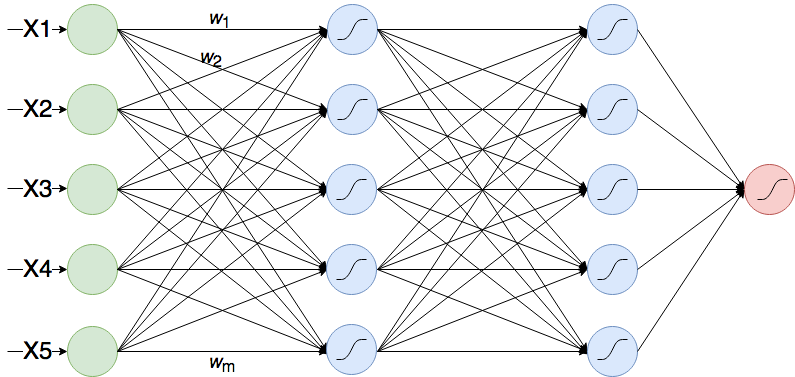
\includegraphics[scale = .37]{ANN}
\caption{Structure of a Feed Forward Artificial Neural Network. Green nodes: input features. Blue nodes: hidden nodes and hidden layers, and a logistic activation function. Red nodes: response vector (the output) and a logistic function.} 
\end{figure}
One model I chose to implement was a feed forward artificial neural network (FFANN). Based on the research conducted in Section 2.1, their results proved to be more than adequate for this problem.\\
A FFANN usually follows the same layout, which makes them applicable to an array of complex classification problems. The basic structure of the ANN can be seen in Figure 1, consisting of an input layer, hidden layer(s) and an output layer. The input layer consists of \textit{feature vectors} representing the data inputs as a single layer of nodes. The hidden layer(s) consists of hidden nodes, used to help alter the representation of the data by transforming it, reducing any nonlinearities in the data. The output is a \textit{response vector} that consists of a single node, which will output the predicted classification. Connecting the nodes in each layer is accomplished using weighted neural synapses, which connect each node in the current layer to each node in the next layer. 

Since ANNs have been used numerous times for this problem, the FFANN was designed to be a benchmark for predictive accuracy on this particular dataset, which could then be compared against the GP that was later developed. 
\subsubsection{Input Layer and Synaptic Weights}\label{subsubsec:inputLayer}
Since ANNs can cope with high dimensional, nonlinear data, I decided to use all 5 KPI ratios as the input feature vectors from the dataset, as the ANN would be more than capable to handle all this data at once.

Due to the stochastic nature of an ANN, when initialising the network before the data from the input features are read into the network, the synaptic weights needed to be initialised. As part of the design, I chose to randomise the weights on each of the synapses. If the weights were not initialised randomly, when the network learns, it would learn in the exact same way every time the program is run because the network will always start at the same position in the search space. This means it will always follow the same routine to get to a solution which would always be the same since it would be predictable.  By initialising the weights randomly, the symmetry of the network is broken, which allows the network to be initialised differently, so the weighted input signal that moves from one layer to the next would always be different. This would allow more of the search space to be explored, and more, possibly optimal, solutions to be found.
\subsubsection{Hidden Layers and Activation Function}\label{subsubsec:hiddenL}
Figure 1 shows an example of a FFANN with a (2,5,5,1) structure. Through my research, it was found that when using one hidden layer with multiple nodes, the network would be more likely to start memorising the data being passed to it, which could cause the model overfit the data \cite{ref-nine}. This means that when testing the predictive accuracy of the hold-out data, the results would be poor as it would be unable to generalise the model. To avoid this, I hypothesised that by using multiple hidden layers initially, the network would generalise better without network memorisation. To make it easier for the user to input their own ANN structure, I decided to provide a configuration file for custom FFANN configuration to allow a user to input their own structure. 

Each neurone in the hidden layer transforms the values from the previous layer with a weighted linear summation. The cumulative sum of these products (\textit{z}) is used as input to the next node in the hidden layer, which then is then passed through a nonlinear activation function. For the ANN that was being designed, I initially used a \textit{logistic activation function}, as indicated by the logistic curves in each of the hidden nodes in Figure 1 and equation 1. \begin{equation} activationL(z) = 1/1+e^{-z} \end{equation}
The logistic function adds an element of nonlinearity to the model, allowing the computation of nontrivial problems using only a small number of nodes, making this function much more popular relative to other activation functions like a \textit{step function}.
\subsubsection{Output Layer and Learning Mechanism}\label{subsubsec:output}
The output layer receives values from the final hidden layer and transforms them into output values. I planned to classify the outputs as either a 0 or 1 by passing the raw output through another logistic activation function. If the new value was below 0.5, then it was classified as 0, otherwise 1. Using this, the error percentage could be measured against the true data classifications, and the weights on the synapses would be altered accordingly using a learning mechanism. For this model, a \textit{back-propagation} learning mechanism was needed to allow the network to learn, and try to minimise the error rate by manipulating the weights on the synapses. This would give the best possible accuracy and show that the network has trained.
\subsection{Genetic Program Design}\label{subsec:gpDes}
\begin{figure}[h]
\centering
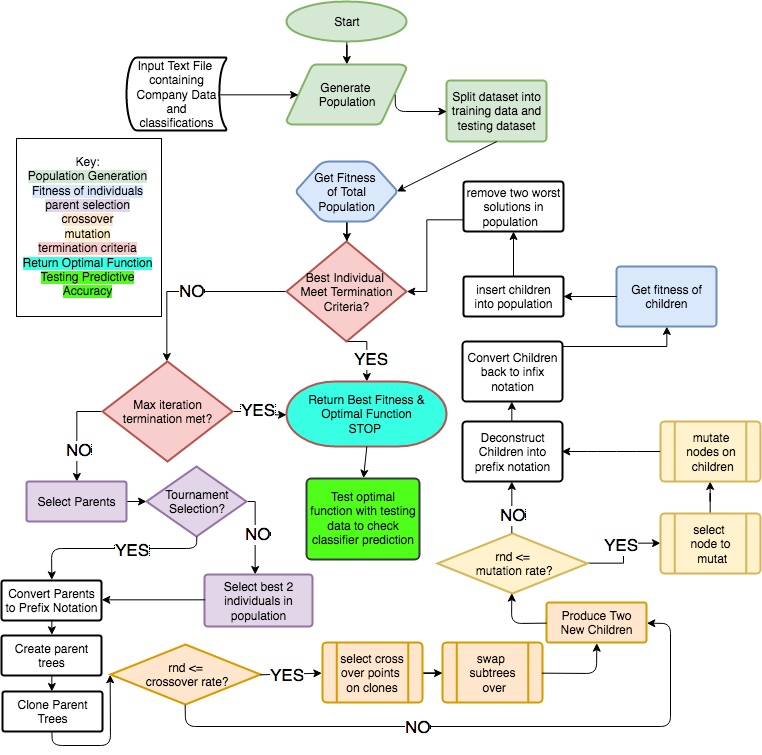
\includegraphics[scale = .55]{GPFlowReformat} 
\caption{Flow chart to represent the Genetic Program that was designed. Dark green boxes: population generation. Red boxes: termination criteria. Purple boxes: selection methods. Orange Boxes: genetic crossover. Yellow boxes: genetic Mutation. Blue boxes: fitness function. Turquoise box: optimal function returned. Light green box: use of optimal function on testing data set.} 
\end{figure}
The aim of the GP model was to produce an optimal function which can predict to a degree of accuracy, whether a company is likely to go bankrupt or not within one year, based on unknown input data. As this type of model was known to be able to handle noisy and nonlinear data well, I decided to use all the 5 KPI ratios for the inputs; the same inputs for the ANN. This allowed for data consistency and would make the models more comparable in the testing phase.
\subsubsection{Data Representation}\label{subsubsec:dataRep}
Throughout this project, each member of the population had to have some form of representation. Here, I mention some of the ways that the data could be represented which I planned to implement in section 4. 

An example of a random population generated containing 4 members can be seen below in the variable \textit{pop\textunderscore n}. Each member is represented as a string, using standard infix notation; the entire population is stored within a list. Infix notation is the format expressions tend to be written in, where 2 operands surround an operator. The reason for this is because when an optimal function is found, it would be returned as a mathematical function, typically represented in this particular format. 
\begin{align*}
pop_n = [``X1+1.3-X3+X2/X4*X5" ,``X2/X5+(6.433-X1)*X3*X4", \\
``X1*9.56-(X2*(X5*X4))-X3", ``4+8.22/X1*X2-7+X3/X4*X5"] 
\end{align*}
To make the \textit{crossover} and \textit{mutation} process simpler, I decided to represent the parents using lazy instantiation of a \textit{binary expression tree} data structure. Lazy instantiation is the process of performing an action only when required. Binary trees make the process of genetic crossover and mutation significantly easier, as the model learns as they can perform insertions and deletions of elements efficiently. I decided to use lazy instantiation because it saves computation time by not having to generate binary trees for every single member of the population, even though only the two selected parents will be going through the genetic operators to create children. Figure 3 is an example of two expressions converted into binary trees. After the processes of genetic crossover and mutation are completed, the children need to be put back into the population, if they are fitter than the worst members of the population. Therefore, since the children have to be in the infix format, the binary trees have to be parsed back into an infix notation which the population will accept. Please refer to Section 3, sebsection 3.5 to gain a better understanding of \textit{crossover} and \textit{mutation}.
\begin{figure}[h]
\centering
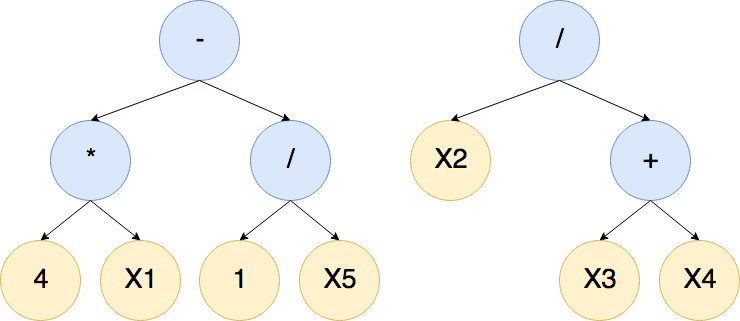
\includegraphics[scale = .40]{binaryT}
\caption{Infix expressions: ``4*X1-1/X5" and ``X2/(X3+X4)" converted into binary trees. Blue nodes: operators. Yellow nodes: operands. } 
\end{figure}
\subsubsection{Generating a Population}\label{subsubsec:genPo}
It is common practise to initialise a population randomly in GPs. The reason for this is to allow different populations to begin in different parts of the search space, such that they can explore different areas to try to find the global optimum solution, which in this case would be the optimal function.  This population would consist of randomly created mathematical functions, each representing one member of the population. A mathematical function typically consists of two parts; a \textit{functional set} of operators (\textit{+,-,*,/}) and a \textit{terminal set} of operands (numerical constants and variables \textit{X1,...,X5}). To create a random member, I decided to design a mathematical expression generator. This would allow random, valid functions to be created using randomly selected members of the functional and terminal sets and would represent an individual's \textit{genotype} - the elements that make up the function. To begin with, a population would consist of 500 randomly generated individuals. Based on the arities of the functional operators, the randomly generated population was based on the \textit{full} method of population generation \cite{ref-book}, rather than \textit{grow} or \textit{ramped half and half} \cite{ref-koz}. This provided sufficient variety in expression generation.
\subsubsection{Fitness Function}\label{subsubsec:fp}
The fitness function represented the \textit{phenotype} of an individual, that is, how good the individual was suited to its environment, representing how close it was to an optimal solution. This was done through calculating the error between the true classifications of the data set and the predicted output as given by the function produced. The aim of this was to minimise the error between the actual classifications from the dataset and the number of incorrectly predicted classifications produced by the function where the optimal function which correctly classified every company would have a fitness value of 0. This could be called a minimisation problem where the objective was to minimise the fitness function. 

For this, I used the \textit{Number of Hits} fitness function \cite{ref-twelve} . This fitness function was calculated by passing each row of data through the function. For each row, the output was either a positive or negative number given by this function. This output was then passed through a \textit{logistic} function. If the value was greater than 0.5, it would be classified as 1, otherwise 0. Using these classifications for each predicted row of data, these could now be compared against each of the true classifications from the data. For every row of data that was classified correctly, the fitness value did not increase. However, for every misclassification, the fitness value for that function increased by 1. This shows that a good function which has more number of hits would have a lower fitness value, and a function which has a high misclassification rate has a high fitness value. 
\subsubsection{Selection}\label{subsubsec:selection}
The better the individual is in the population, the more likely they were to be selected to produce children functions. To select these parents, I chose to use \textit{tournament selection} \cite{ref-book}. This works by selecting a random subset of the population, \textit{t}, and then comparing the fitness of each of the members of \textit{t}. The individual with the best fitness value i.e. closest fitness to 0, will be selected as the first parent. This same process will occur to select the second parent. An individual can only be selected once per generation, as the same member of the population cannot be selected to be both parents. This will keep the selection pressure relatively constant as it does not favour the best individuals in the population, rather it selects the best individuals from the subset of candidate parents. The reason this method was chosen was to help reduce selection pressure, which favours the very best individuals. By reducing this, it enables more members to be selected as candidates, and be chosen as parents, even if they were not the best solutions in the population. 
\subsubsection{Genetic Operations}\label{subsubsec:GO}
Using the parents, the children can be created using the genetic operators - \textit{crossover} and \textit{mutation}. Typically, in a GP, crossover occurs first. I decided to use a \textit{single subtree} crossover between the parents, to create two children, each containing characteristics of both parents.
After the two new children have been created, the \textit{mutation} operator can be used to mutate nodes on the children. This was used to help maintain genetic diversity within the population from the current generation to the next. Here, I decied to use \textit{node replacement} mutation, where a random node on each of the children would be selected and altered based on its arity. For example, if the node selected is a numerical value, with an arity of 1, this will be replaced by another value with an arity of 1. Similarly if the node selected has an arity of 2, then it will be replaced by another functional node.
\subsubsection{Termination Criteria}\label{subsubsec:TC}
The termination criteria were checked in two places. The first termination criterion was whether an optimal function had been found in the population. Since there was a possibility of this occurring when the initial population was evaluated, this was checked before the program GP continued. If an optimal solution existed, then this could be tried on the testing data set immediately. After \textit{g} generations of running the program, if the best individual in the population still had not been able to meet the optimal fitness criteria, then the GP should stop and return the fittest individual in the current population, as this would have a fitness value closest to 0 compared to all others in the population. 

Using the optimal function obtained, it could be tested on the hold-out dataset to determine the predictive accuracy of the function in order to see if it has predicted whether a company is likely go bankrupt correctly. This output would then be passed through the same logistic function (eq. 1) using a 0.5 threshold. If the value outputted from this function is greater than 0.5, it would be classified as 1, otherwise 0. This could then be used to give the classification predictive accuracy of the function. The reason this was done was because when training the model, to ensure consistency in the predicted classifications, the thresholds were kept the same. 
\subsection{Testing Design}\label{subsec:TD}
After the development was completed, various tests could be conducted on both the ANN and GP to see if these would alter the learning process and predictive accuracy which will be mentioned now and in the testing phase of the dissertation (section 5). The design of the tests has been based on the project specification and on the way the models have been developed. 
The first type of testing I chose to design was manual testing for the ANN and GP. This involved running the models' multiple times with smaller datasets with already accepted solutions. This was able to check whether the models were working and performing as they should be. 

During the development of the program, I decided to use software testing to determine whether the functions that are being made are functioning in the correct way. After this, I could then perform validation testing by running the models multiple times to ensure that they are both learning the way they should be, to get to an optimal result .To do this, \textit{unit} testing, and \textit{black-box} testing could be used to determine whether each function performs the way it should, by comparing the desired output of the function to the actual output of the function, and checking whether they match.

 After this, performance testing were completed on both models, to ensure that they are learning and predicting at an acceptable rate. This was completed by testing the performance of each function and the overall model to identify the areas of the model which may perform unusually slow. Finally, after the development and testing has completed, \textit{user acceptance} testing was designed to ensure that the program works and could be used as a product that could be deployed in the future. 
\subsection{Programming Language and Environment}\label{subsec:PLE}
The final part of the design stage was to determine what programming language and programming environment could be used for this project. Through careful consideration, I decided to use Python as my main programming language. The main reasons for this were that since the ANN was going to be used as a benchmark, rather than trying to implement an ANN from scratch, I chose to find a library - \textit{sklearn}. This provided all the functionality to allow a FFANN with back propagation methods to be created, along with many other functions which could be used to test the network, for example, using other transfer functions, methods of splitting the data and how to train and test the network. For consistency, I also decided to use Python as the choice of language for the expression tree GP. This was due to the fact that Python offers object orientation, speed, high level abstraction for memory allocation. Furthermore, it offered optimised mathematical libraries such as \textit{numpy} which can make data handing easier, and Matplotlib  - a graphical library which could be used to visualise the results. 
\section{Development}\label{subsubsec:DEV}
To begin with, I developed the models by attempting to solve smaller problems first, with static data. In this way, debugging and understanding the errors would be easier. To make the testing of the models more reliable, I decided to use the same dataset for the ANN and the GP. 

Since the dataset was the same for both models, I used the same method to read and split the data sets from their associated classifications. As this was a SL problem, the decision to split the data was because the classifications from the dataset could be used to form the fitness functions for both techniques implemented.
\subsection{Development of the Artificial Neural Network}\label{subsec:devANN}
As part of the design stage, I chose to use a library in Python - \textit{Sklearn}, a well-known machine learning library that has the facilities to develop a FFANN efficiently, the ability to train, test, and present the outputs of the data in a variety of ways. 
\subsubsection{Multi Layer Perceptron Classifier}\label{subsubsec:MLP}
To initially read the data, a function \textit{read\textunderscore data} was used. This took the dataset, shuffled it, and then split the dataset such that the data was stored in a variable \textit{data\textunderscore CBD} and the classification labels associated with each row of the data stored in \textit{class\textunderscore labels\textunderscore CBD}. To maintain type consistency, since the data was read and stored using the \textit{numpy} module, the classification array was cast to a \textit{numpy} array. 

Next, in order to train the model I made a function called \textit{split\textunderscore data}. This took the data, and their associated labels and allowed the user to determine how much of the data should be used for training the model, and how much should be used for testing the model. To do this, the \textit{train\textunderscore test\textunderscore split} class was imported, which would randomly split the data and their labels into a training and testing set, based on the train and test size parameters. 

To train and test the model, rather than using two separate functions, I used a function called \textit{run\textunderscore classifer}. This used the training data and its classification labels, the user defined FFANN structure as well as the type of activation and learning methods to use, along with the maximum number of iterations for the model to run once. Using the \textit{sklearn.neural\textunderscore network} module, I imported the \textit{MLPClassifer} class. Using the \textit{MLPClassifier} constructor, I chose to use the \textit{logistic} function as the activation function. This is the most population activation to use on feed forward ANNs and part of the project design. On top of this,  I also chose to use the \textit{lbfgs} back propagation technique to make the model learn.

As part of this constructor, the weights on the synapses of the network are initialised randomly when the model is created by default. Therefore, this did not have to be accounted for explicitly. 
To ensure that complex models which would have a high training accuracy were not favoured, I chose to also use a regularisation parameter \textit{L2}. A regularisation parameter is used to penalise networks that are more complex. Complex models may train networks well, but have tendency to over-fit the data, which means they will have poor regularisation. In turn, the model will have a poor classification predictive accuracy. 

The final parameter used for the \textit{MLPClassifier} constructor was the \textit{hidden\textunderscore layer\textunderscore sizes}. Based on the research conducted and as part of the design stage, I chose to make a configuration file, to allow a user to input their own ANN structure. This allows more people to easily use the model, without having to directly edit the source code. For instructions on how to use the configuration file, please refer to Appendix B or to \textit{Configuration\textunderscore file\textunderscore README.txt}.

As many of the crucial functions required to make the ANN were prebuilt as part of the \textit{Sklearn} library, it was computationally efficient in terms of time to develop the model, to allow more time for testing and evaluating the model using the main dataset. 
\subsection{Developing the Genetic Program}\label{subsec:DEVGP}
Like the ANN, a small subset of the dataset was used to begin with. Whilst developing this model, I worked on smaller problems with inputs and outputs that I knew would work, as well as an optimal function which the smaller model could find. The reason for this was to ensure that whilst developing the smaller program, the structure would be developed correctly, and debugging functions through the development phase would be easily traceable. It also meant that if the structure of the model was appropriate, then scaling the model to work with the main dataset would not be problematic. 
\subsubsection{Generating and Handling the Population}\label{subsubsec:sf}
The first stage in the development process was to create a population of functions based on the functional, terminal sets, and population size as set out in the design specification (Section 3). To do this, I created a class called \textit{GenMember}. The purpose of this class was to handle a population by generating all the members, finding their fitnesses, selecting the parents and updating the population. By encapsulating the functions within a class, this helped to improve the structure and usability of the model. 

The first function, \textit{generate\textunderscore expression}, was used to generate random mathematical functions in infix notation using recursion. Recursion allowed multiple sub expressions to be created which could be concatenated together to build full, valid functions. 
As the size of the functions increased, the time it took to evaluate and manipulate the functions increased, therefore to ensure that that the function stayed a reasonable length, a \textit{max\textunderscore depth} parameter was imposed.

Using the project design for the population generation, I used the \textit{full method} \cite{ref-koz} of function generation to provide sufficient variety in the size of each of the functions produced, based on the maximum depth limit. This allowed the functions made to be sufficiently organic but still controlled. 
Unfortunately, since functions did not necessarily contain all 5 KPI ratios, I created the function - \textit{get\textunderscore valid\textunderscore expressions}, which filtered out and replaced any invalid functions with valid ones which contained all 5 KPIs at least once. 

Next, each member had to be evaluated to determine how close to an optimal fitness the member was. \textit{get\textunderscore fitness} was called in two scenarios - when the population is initially created and when a new child is produced. When the population was initially generated, all the individuals needed to be evaluated, as an optimal expression may exist within the original population. To evaluate each member, each row of the sample data is fed into the population of expressions, and the total was found. This number was then passed through a \textit{logistic function}. If  the output was below 0.5, it was classified as 0, otherwise 1. Using this, the actual classification labels from the dataset were then compared to the predicted classification labels. For every incorrect prediction, the fitness error value would increase by 1. Very poor solutions had a very high fitness value, whereas very good individuals with strong predictive accuracy had a very low fitness value as the aim was to minimise the error to produce an optimal function.\\

Using the evaluated population, the parents needed to be selected. To accomplish this, I made the \textit{tournament\textunderscore selection} function. The output of this function would be the two individuals selected to produce children through crossover and mutation. 
The population and their associated fitnesses were inputted, as well as a user defined tournament selection size. The size refers to the number of candidates that would be selected from the population, as potential parents. The two individuals that were the best from each tournament would then be selected as the parents. The population and their associated fitness's were zipped together to prevent a member obtaining the wrong associated fitness value. Based on the \textit{selection\textunderscore size}, \textit{``c"} candidates were selected randomly from within the population. As two parents are needed for the process of crossover to occur, two tournaments were completed to select both parents. To ensure that exactly one parent from the population was selected each time, the first chosen parent was popped out of the population to prevent the same individual being selected twice. 
\subsubsection{Infix to Prefix Conversion}\label{subsubsec:I2P}
\begin{equation}parents = [(``X1+1.3-X3+X2/X4*X5",170),( ``X2/X5+6.433-X1*X3*X4",243)] \end{equation} \begin{equation}parents = [([``+", ``X1", ``-", ``1.3", ``+", ``X3", ``/", ``X2", ``*", ``X4", ``X5"], 170),([...],243)] \end{equation}
The selected parents could now be put into a binary tree structure. Attempting infix to binary tree conversion proved to be much harder than anticipated. Through further research into how to convert infix notation to binary trees, it was found that a further step was needed to make this process more manageable \cite{ref-pre}. This step involved converting the infix notation into \textit{prefix} (\textit{Polish}) notation. This format is easier for the machine to parse into a tree structure. For this, I used a class called \textit{ToPrefixParser}. Each parent was split into their individual elements. To ensure that each component of the parent was split correctly, I used regular expressions to split the strings.
Using an online guide \cite{ref-pre}, I manipulated a subset of their functions to convert the infix notation into prefix notation, as this website was not enough by itself. The \textit{get\textunderscore operation}  function was used to compare the \textit{0th} element of the expression that is being passed in to the \textit{expected character} that the parser was looking for. If they matched, then the value was popped out of the original expression. The \textit{expected character} was checked throughout the other parsing functions. The \textit{is\textunderscore number} function is used to return a number which is a leaf value. 
However, if the character being checked is a ``(" and the expected character is also a ``(", then this will call the \textit{get\textunderscore expression} function which, in turn, would be used to get the subexpression that exists within the pair of parentheses. The reason for this is that prefix notation and binary trees do not use parentheses, as the full structure of the function is changed. When \textit{get\textunderscore expression} is called,  a chain of other functions is called sequentially, which will put the infix notation into prefix notation.
\textit{get\textunderscore expression} calls the \textit{get\textunderscore product} function, which then calls the \textit{is\textunderscore number} function which checks to see if the current character being checked is a ``(", in which case the sub-expression is then evaluated, otherwise a number is added to the prefix notation output stack.  As each character in the infix notation was checked, these functions were called to correctly convert the infix notation into prefix notation. \\ 
After both parents were converted from infix to prefix notation, the newly converted parents were returned by the \textit{get\textunderscore prefix\textunderscore notation} function.  

As seen from Section 3.3.1, Figure 3, a binary tree consisted of multiple nodes, which were linked together. In turn, the next class  developed was the \textit{Node} class. 
\subsubsection{The Node class}\label{subsubsec:node}
 A binary tree consists of two types of nodes; \textit{branch nodes} and \textit{leaf nodes}. Branch nodes hold a value, and have ``left" and ``right" child references. Leaf nodes hold a value, but have no child references. Both branch and leaf nodes have parent nodes. The top of a binary tree is called the root node, which is a branch node; however, it is unable to hold a reference to a parent as it is the eldest generation. Multiple nodes that are connected form a tree. This can be seen in Figure 3.  
 
Based on the structure of what a node can hold, the \textit{Node} class was developed, encapsulating 4 functions. The first function was the constructor, which held the attributes that a node object could hold. These include the current node value, the possibility of holding references to a left and right child, the possibility of holding a reference to a parent node, and a nodeID, which assigns a unique number to each node as they are created.
Each node was null until a value and nodeID was assigned to it, which was completed when the tree was constructed. The second function was the ability to add a child node. This function took a value and either inserted a child into the parent's left or right branch depending on the current state of the ``left" branch. Every time a new child was added, the child also held a reference to its direct parent to indicate that the child is connected to that one specific parent.
 
The final two functions used gave a visual representation of exactly how a tree would look. Examples of this can be seen in Appendix C. 
\subsubsection{The Tree Object}\label{subsubsec:tree}
The tree representation of each parent could now be built using their prefix expression. The \textit{Tree} constructor contained a root node, as this is how all trees need to begin. \textit{make\textunderscore tree} was used to build the tree. To initialise the tree with a root node, the first index of the prefix expression was removed and assigned as the root node. To track the nodes, I used a \textit{current\textunderscore node} variable initially set to the root node.
The value was removed from the parent prefix list as it was no longer needed. Based on the current node selected, a check was needed to see whether the value was within the functional set of values. If the current node was a functional operator,  it would have exactly two children, a left and a right child. Therefore, I performed a check to see if the left child for that node had been created. If it was empty, then the next value in the prefix list was inserted into the left child and the left child became the new \textit{current\textunderscore node}. If the current node was a leaf node from the terminal set of values, then it could not have any more children. In turn, the parent's right branch was checked. If the right child was empty, the tree would continue to be constructed via this route. Otherwise, one would move back up the tree to the root node and then start building the tree to root node's right child to build the rest of the tree. After all the prefix list was empty, the tree had been built and was then returned. 

It was necessary for the root node to be returned, due to the fact that this had access to all the children, which make up the full tree. Therefore, every node could be accessed from here. A list of nodes was returned to show all the subtrees of the tree, as this allowed accessing the nodes for crossover and mutation to be easier. Finally, another variable \textit{nodenums} was returned which was used to track the nodeID of each node in a tree. As each node was created, it was assigned an ID value. I made the nodeID variable static such that regardless of what tree is made, the value of the ID would always increment by 1. The reason for this was because when performing crossover and mutations on the tree, I would not have to reassign the nodeIDs to the new trees, they could keep their original nodeID's.
\subsubsection{Crossover and Mutation}\label{subsubsec:CM}
Through the process of \textit{crossover} and \textit{mutation}, two new children were created, containing certain characteristics of both parents. Since I wanted to keep the parents in the population before starting this process, I used a \textit{deep clone} function to clone both of the parents. This allowed for the parent clones to be completely independent from the original parents. These clones could be used to create the children. In this way the parents were not effected, and two children trees were produced. \\

I chose to complete a \textit{subtree crossover} based on the design stage. Here, three functions were created; firstly, \textit{select\textunderscore random\textunderscore val}. This selected a random subtree from the list of possible nodes. The node selected and its entire subtree would therefore be encapsulated within this. When selecting the node at random, I removed the root from this selection. This was because every node is a subtree of the root node, which means if crossing over occurred, then the full tree would be crossed over and this was prone to errors. \\

To ensure that the subtree did exist in the tree - \textit{find\textunderscore subtree} located the subtree within the parent. This function took three parameters; the tree itself, which would be searched, secondly, the list of nodes as this is where the random value had been selected, and the random subtree would be selected from this. The last parameter to this function was the nodeID. To search for the subtree within the parent, I implemented a recursive depth first search. If the depth first function located the node value, it would then also check the nodeID to ensure that this was the correct node to be selected. If the subtree was found, it was returned.

Subsequently, the main crossover function \textit{swap\textunderscore nodes} was made. The purpose of this function was to simulate genetic crossover between the two parents, as this would create the children. To begin, the parent of the node to be swapped was checked. This was to determine whether the subtree selected belongs to the parents left or right child and ensured that the correct subtree is being swapped over as the parent association with the current child subtree was reassigned to the new child that is being reassigned from the other parent. By doing this, the parent nodes now had different child nodes, indicating that the crossover had been achieved successfully. An example of this may be seen in Appendix C for a diagrammatic representation of crossover. 

Once the crossover was performed, the ``parent clones" were considered to be the children of the original parents as each new tree contained characteristic from both parents. As crossovers were more likely to cause bigger changes when searching the search space, it was recommended that crossover should not occur during every single epoch \cite{ref-book}. Therefore, I used a crossover rate which can be defined by the user as a value between 0 and 1, where the user can select how frequently they want crossover to occur. When the cross over rate is low, there is a greater likelihood of crossover not occurring. When crossover did not occur, the parent clones remained exactly the same and progress to the next stage of mutation. \\

Although the children trees were built, the list of nodes that they each possessed had not been updated. The issue with this was that to select a random node to mutate, and to find the subtree, this required using the selected members list of nodes. Therefore before going the process of mutation, the children's list of nodes had to be created which could then be accepted by the \textit{select\textunderscore random\textunderscore val} and \textit{find\textunderscore subtree} function. This was the reason for the creation of \textit{make\textunderscore list\textunderscore nodes}. 

Following this, the \textit{mutate\textunderscore node} function was created. This function considered the tree to be mutated, the list of nodes it held, and the random node to be mutated. The function also checked to see what type of value has been selected to be mutated, that is, whether it is a functional, variable or numerical node value. If it was from the functional set, then it randomly selected another value from the functional set with the same arity. However, if the value is from the terminal set, then another check is performed to see if the value is a variable X1,..., X5 or a numerical value. If the value is a numerical value, based on a random Gaussian normally distributed value, the mutation will cause the node to be altered by a certain amount. However, if the selected node was a variable, then it would randomly select another variable instead. Therefore, this was known as a \textit{node replacement} mutation \cite{ref-book}. Whichever value was mutated automatically updates the tree and updates the list of nodes accordingly, to ensure that the newly created child is consistent with all the changes that have occurred. Like to the crossover rate, mutations are not meant to necessarily occur during every epoch, therefore a mutation rate was used, which again, will be defined by the user, which will be defined by the user, but by default is set to 0.1, such that mutations would only occur 10\% of the time.
\subsubsection{Prefix to Infix Conversion}\label{subsubsec:P2I}
Once the children had been created, they needed to be evaluated again and reverted to a state that the population would accept. This meant making a class \textit{ToInfixParser} to convert the child tree representation back to infix notation. 
\textit{ToInfixParser} contained two methods, which would convert the trees into infix notation. \textit{deconstruct\textunderscore tree} took the nodes from the child list of nodes, and extracted the values from the list, to return it back into the prefix notation state. 
\textit{conv\textunderscore infix} took the prefix list, and went through each of the values in the prefix list backwards, starting at index -1. For every value that was not an operator, it added the value to a stack. If an operator is encountered, it popped the values currently in the stack and put the current sub- expression into a bracketed form - ``(\textlangle{}operand1\textrangle{}\textlangle{}operator\textrangle{}\textlangle{}operand2\textrangle{})". This started to build the full expression back the infix notation, which was now in a state that the original population could accept.
\subsubsection{Updating The population}\label{subsubsec:UP}
The next step was to find the children fitnesses, using the same \textit{get\textunderscore fitness} function. Since this was a child expression, when \textit{get\textunderscore fitness} was called, the default \textit{child} Boolean variable changed to true, such that the child expression was parsed into an acceptable format that would allow \textit{get\textunderscore fitness} to return the fitness to the same state as when the population was originally evaluated. The reason that only the children had to be evaluated is that the rest of the population had already been evaluated in the current population, and a re-evaluation would waste computational time.  \\

Once the children fitnesses had been found, the population could be updated accordingly using \textit{update\textunderscore population}. This function took the original population and the new child, and compared the new child against the worst member in the current population. If the child was better than the current worst member of the population, the child replaced the worst member in the population. This process is repeated for the second child, to ensure that the worst members of the population were filtered out, and to enable the GP to learn, by accepting better, fitter individuals and rejecting those that are worse. By replacing one individual at a time, this also helped to make sure that the population size remained the same as when it started. 
\subsubsection{Training and Termination}\label{subsubsec:TR}
After implementing the classes and subroutines based on the design specification and initial project specification, the GP model had been built. The final step of development was to create the function to put everything together. This was the \textit{run} function, where the model could be executed at once. For this, a \textit{train\textunderscore gp} function was created, which is where the model would learn, to produce the optimal function to predict CB. Since the \textit{train\textunderscore gp} function was where the model would learn, this function contained multiple tuneable parameters. The reason for this is that when testing the code, rather than having to search for every parameter that can be changed, I only had to change the value in the definition of the function.

Within the \textit{train\textunderscore gp} function, the initial population was generated exactly once, and entered a loop where the model began to learn. The significance of this loop relates to one of the termination criteria - \textit{max\textunderscore iteration}. The model starts by evaluating the population once, and checks to see if an optimal solution already exists in the original population. If the original fitness is smaller than or equal to 133, then this has met the termination criteria as the function would have at least 75\% training accuracy. The second termination criteria was met if the user defined maximum number of iterations were reached. 

Once the termination was met, the optimal function was then returned and was used to test the predictive accuracy of hold-out data to see if it was able to accurately classify the hold-out sample data correctly. \\

After executing this model multiple times, \textit{optFunc} and \textit{optFunc2} show examples of optimal functions that were produced, which gave 75\% and 76\% predictive accuracies on the hold-out sets respectively.  These two examples have been manually pruned to fit onto the page, as the functions were much larger. 
\begin{align*}
optFunc1=  35.400318494530815+(X3-X2-(673.1926*X2*X4^4*\\
X5^2+8.7779947854)-25.99600428294065*X4^3*X5) = 75\%  accuracy
\end{align*}
\begin{align*}
optFunc2 = X3*(X3+(((X4*(X2/((X4*(3X4-X1-X3))-\\
X2)))-X2)-X1+X4))-X2-X5-X1+X4 = 76\%  accuracy
\end{align*}

Overall, using my research and following the design specification, the ANN and GP had been successfully developed. To run both models, I chose to use rough parameters to allow both models to learn, and then test the predictive accuracy of each model with these parameters. Once both models were developed, I then scaled them, such that they could both accept the full dataset that was to be used for training and testing the predictive accuracies of both models. I was aware that the parameters used were not necessarily the most optimal, and therefore I decided to run a variety of different tests which will be discussed in the following section.

To run the GP, please look at Appendix C which shows you how to execute the file using the configuration file. 
\section{Testing, Results and Comparisons} \label{sec:TRC}
\subsection{Testing and Results}\label{subsec:TnR}
I used various methods to test whether the code was performing the way it should, and to see if different techniques affected the training and testing predictive accuracy of both the models. For both classification models, I created a testing plan which was split into two sections for both models. The first section of the plan related to \textit{software testing}, to check if each function was performing as it should. The second section of both plans related to testing whether or not the models made were classifying the data correctly and to change parameters to see if this affected the training and testing predictive accuracies. Within this section, I discuss some of the methods I used to perform different types of testing such as \textit{\textit{black box}, unit, and performance testing}. I then mention some of the completed experiments through parameter tuning, to get optimal predictive accuracies. 
%%%%%%%%%%%%%%%%%%%%%%%%%%%%%%%%%%%%%%%%%%%%%%%%%%%%%%%%%%%%%%%%%%%%%%%%%%%%%
%%%%%%%%%%%%%%%%%%%%%%%%%%%%%%%%%%%%%%%%%%%%%%%%%%%%%%%%%%%%%%%%%%%%%%%%%%%%%
\subsubsection{Code Functionality and Parameter Tuning: Artificial Neural Network}\label{subsubsec:CFPT}
Since the feedforward ANN was created using \textit{Sklearn} - it did not seem necessary to perform software testing to determine if the \textit{MLPClassifer} was functioning correctly. The reason for this was that through reading the \textit{Sklearn} documentation for the \textit{MLPClassifier}, the class and its functions that were provided had already been thoroughly tested before being deployed to the public and made to be user friendly \cite{ref-sklearn,ref-absk}. However, it was possible to test the functions that I created to make sure that the data was being read and passed through functions like \textit{run\textunderscore classifier} to assert that the model was learning on the correct data. On top of this, there were still different ways that the parameters could be modified to result in different predictive accuracies of this model. 

The data was read in and shuffled and split into two sets;  a training set and a hold-out set. The training set was used to train the ANN model by altering the weights of the synapses. The hold-out set was used evaluate the predictive performance of the model using unforeseen data. This method is called \textit{train\textunderscore test\textunderscore split} (TTS). The benefit of splitting the datasets is that the hold-out accuracy rewards simpler models, as they tend to generalise better. Splitting the data into these two sets also helps to prevent the overfitting of the model. This tends to occur when the whole dataset has learnt perfectly when training the model due to memorisation, and in turn is unlikely to generalise to future data.
Within the TTS constructor, I chose to use a (5, 5, 5, 1) structure to train the model. This was based on the design and project specification that was originally set out. Within this constructor, I chose to vary the training and testing set sizes, to determine how much data the network needed to train on to output a solution that produced the best classification accuracy. This can be seen in Figure 4. 

The drawback of using TTS is that the testing accuracy is a high variance estimate hold-out sample accuracy. This means that every time a new random subset  of data is being used to train and test the model,  the network will train differently every time it is run as the observed values in the training set will differ each time. This is a major drawback to TTS, even if the parameters remain constant. 
This issue can be seen throughout the Figure 4, as the variance of using 10\% and  90\% of the data to train the model, ranged from 6.8 to 35.2 respectively.  Another reason that a large variance may occur is because this is a \textit{non-deterministic} model to begin with. Every time a new instance of the model is created, the weights on the synapses are initialised differently. As a result, different areas of the search space will be explored using a learning algorithm to try to find an optimal solution. 
I decided to use 80\% of the dataset to train the model and 20\% to test the model. The reason for this is that if 90\% or more data was used to train the model, there would be greater likelihood of the model overfitting the data. Conversely, 10\% or less was chosen to train the data, then there was a strong likelihood of the network under-fitting the data. This would be because the model is not sufficiently complex to handle noisy data. This could also, therefore, explain why using 10\% of the data set has a high variance. 

One way that high variance can be reduced is by using \textit{K-Fold Cross-Validation (KFCV)}. The idea here that the \textit{train test split} method is run several times, using different train test splits each time, calculating the hold-out accuracy for each test and then taking an average of all the results to get an average prediction for the model. For this to work, the data is divided into \textit{K} partitions, where \textit{K-1} sets would be used to train the model, and the remaining data is used to validate the model, calculating the predictive accuracy each time. This process is repeated several times, until an average of the validation accuracies of the model is obtained. This average is known as the cross validated out of sample accuracy which can be used as the hold-out accuracy.  The benefit of this method is that here, every data point is used during the training phase and also during the testing phase.

To implement this, I used the \textit{cross\textunderscore val\textunderscore score} class, with 10-Fold Cross Validation containing up to 3 layers. To improve upon the original ANN, as seen in the development stage, even though the user can decide the structure of the ANN, a better model could be used to find the optimal number of nodes and layers for the model itself. As inputting more layers increases the computation time, examples of the optimal nodes found for 1, 2 and 3 layers have been shown in Figure 4b. 

Figure 4b and 4c clearly show that relative to TTS (4a), the variance was reduced. For example, when one hidden layer was used, (5 49 1), this had a variance of 0.00067, which was significantly lower than when using the TTS. Looking at the \textit{Area Under the Curve} (AUC) for each of the three models, they had a minimum of 84\% accuracy, approximately 10\% more accurate when using TTS. Using the Receiver Operator Characteristic (ROC) curve and the area under each curve, this also indicated that the results produced were in fact accurate and not down to ``random luck". When comparing this to the ROC curve produced for the TTS, it becomes clear that using KFCV was a radical improvement on the predictive accuracy, even though this performed slower. 
\begin{figure}[h]
\centering
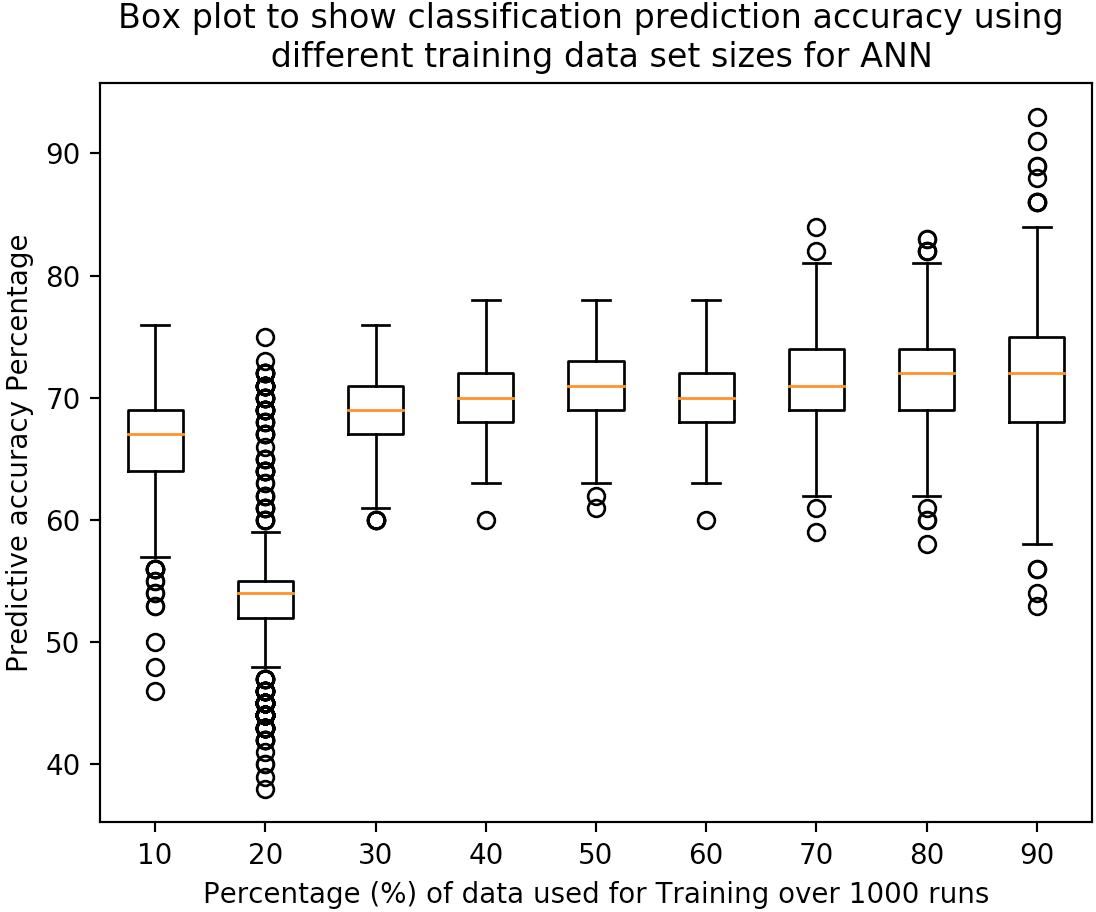
\includegraphics[scale = .40]{optTTS}
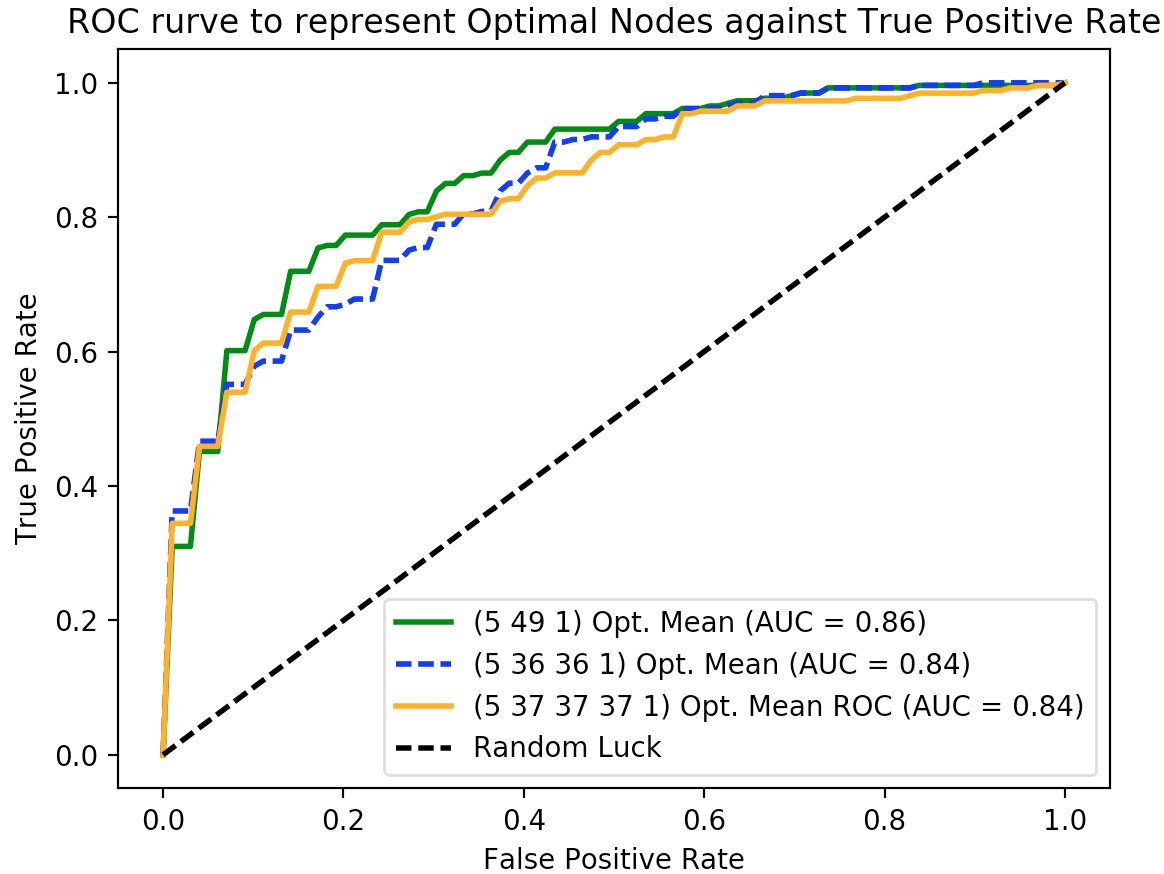
\includegraphics[scale = .40]{roc1}
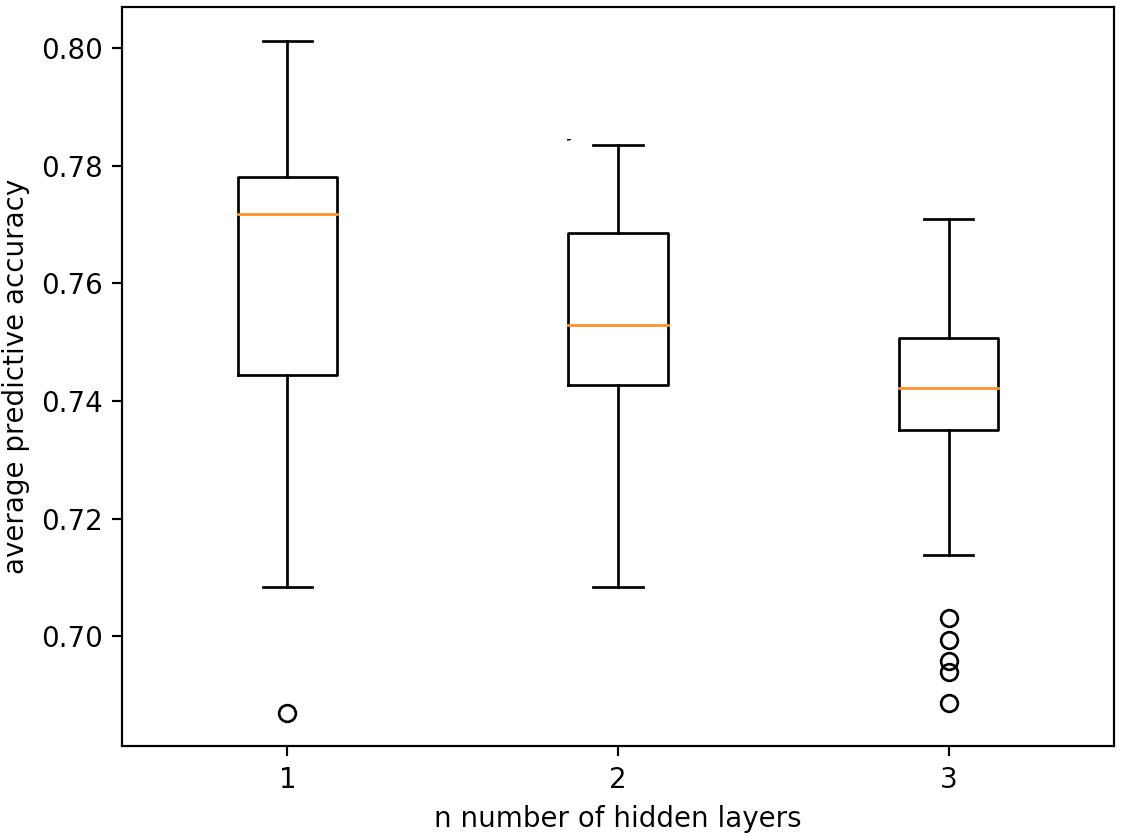
\includegraphics[scale = .40]{reduc}
\caption{(a)Graph shows the use of TTS to get the classification accuracy of the ANN. (b) graph shows the use of 10-Fold cross validation to get the classification accuracy of the ANN. (c) Graph to show the ROC curve to determine algorithm performance. } 
\end{figure}
\subsubsection{Software Testing: Genetic Program}\label{subsubsec:STGP}
I originally generated a small set of static data with classifications, with an optimal function that could be used to verify whether or not the GP was learning when starting GP development.
\textit{GenMember} was used to create random valid mathematical functions, select parents and update the population. Unfortunately, as it was very difficult to test whether \textit{generate\textunderscore expression} was working, manually verification was completed to check if this function was producing valid mathematical functions. To ensure that the \textit{get\textunderscore valid\textunderscore expression} worked, since the generated expression needed to contain all five variables X1,...,X5, the only way that this condition could be checked was to call the function multiple times based on the generation created originally. Using these outputs, I was able to acknowledge that they were correct, and created a small population of 6 individuals. 

Based on the fitness values given to each of the individuals in the population, I performed \textit{Unit testing} on functions such as \textit{tournament\textunderscore selection}, as I knew the sample population. Here, I used \textit{white box} testing within the unit test, to ensure that out of these 6 individuals, 4 were candidates and the best individuals were assigned to be parents. This was tested multiple times with different populations of different sizes to ensure that the best potential candidates were always being selected. 
%%%%%%%%%%%%%%%%%%%%%%%%%%%%%%%%%%%%%%%%%%%%%%%%%%%%%%%%%%%%%%%%%%%%%%%%%%%%%
%%%%%%%%%%%%%%%%%%%%%%%%%%%%%%%%%%%%%%%%%%%%%%%%%%%%%%%%%%%%%%%%%%%%%%%%%%%%%
To enable the infix to prefix conversion to be successful, the state of the infix function had to be changed into an acceptable format for \textit{get\textunderscore prefix\textunderscore notation} to accept. As some of this class was taken from another source, to initially test this on sample problems, I wrote out example infix functions and manually converted them to prefix functions. I used \textit{black box} testing to check whether the infix notation was correctly being converted to prefix notation, on small and larger expressions, to ensure that every expression was being correctly converted. 

Using two expressions (to simulate parents) that were converted into prefix, I was then able to start testing the \textit{Tree} class. For \textit{make\textunderscore tree}, I used a simple prefix expression
and manually constructed what the tree should look like. If the expected tree followed the same structure as the manually drawn tree, i.e. nodes placed in the correct place, and correct associations with their respective parents, then the \textit{make\textunderscore tree} function was functioning correctly (see Figure 3 for an example).  This same process was repeated for larger, more complex prefix expressions, to ensure that this function could build any tree, based on any variety of prefix expression.  

To ensure that \textit{find\textunderscore subtree} was performing effectively, rather than trying to find a random nodeID, I chose to use a specific node in order that I would be able to track the search in a ``verbose" mode. This also meant that I could confirm that it was reaching the expected node at every stage.

Another crucial function that needed testing was \textit{swap\textunderscore nodes}. To test this, I used two prefix expressions which simulated parents in their binary tree structures. By inserting and printing the parents that would be crossed over, it was clear to see that the exchanging of nodes had taken place. Here, \textit{white box} testing was performed to determine that the new children produced were contained in the right nodes and contained the correct nodeIDs. This was relatively straightforward to test as I could print the new tree objects produced and compare the original parents to the children, based on the child nodes that had been selected to be crossed over.  This same process was performed for the \textit{mutate\textunderscore node} function, as they both required the tree inputs, and the node(s) to be manipulated. Therefore, since I selected a specific node to be mutated, I was able to see exactly what it was mutated to, ensuring that this function was performing as expected.\\
%%%%%%%%%%%%%%%%%%%%%%%%%%%%%%%%%%%%%%%%%%%%%%%%%%%%%%%%%%%%%%%%%%%%%%%%%%%%%
%%%%%%%%%%%%%%%%%%%%%%%%%%%%%%%%%%%%%%%%%%%%%%%%%%%%%%%%%%%%%%%%%%%%%%%%%%%%%
The next class that needed testing was the \textit{ToInfixParser} class. Using a simple problem to begin with, I used a prefix notation expression, and manually converted this to infix notation. Using this as the desired output, I used \textit{black box} unit testing to determine if that prefix expression was converted to the same infix expression in the \textit{conv\textunderscore inf}  function . This was repeated multiple times on small and then bigger prefix expressions. To ensure that this was correct, I had to evaluate the newly created infix expressions to ensure that due to the encapsulation of the sub expressions, the numerical value of the function remained the same. If they did, then this test was successful. 

After the children were evaluated, \textit{white box} testing confirmed that the children were in the correct string format to be accepted back into the population. I was able to check where the children were checked against the worst members of the population, see which members of the population were changed, and whether the population sized definitely stayed the same. If the worst members of the population were removed and the population size remained constant, then the model was starting to learn as it was filtering out worse members of the population. 

Finally, the last section to test was the termination criteria. Using a sample population, I was able to track the progress of the population through a few iterations. By keeping the termination criteria very flexible, I could check that if certain conditions were met, the program would terminate successfully with the a function being returned as part of the output. 
%%%%%%%%%%%%%%%%%%%%%%%%%%%%%%%%%%%%%%%%%%%%%%%%%%%%%%%%%%%%%%%%%%%%%%%%%%%%%
%%%%%%%%%%%%%%%%%%%%%%%%%%%%%%%%%%%%%%%%%%%%%%%%%%%%%%%%%%%%%%%%%%%%%%%%%%%%%
\subsubsection{Running the Genetic Program - Training and Testing datasets}\label{subsubsec:RGPTT}
Similar to the ANN, it is very common to train the GP using one dataset and test the predictive classification accuracy on another dataset. During the development of the project, after an optimal function could be found on smaller problems and classified a hold-out sample dataset correctly, I used a random selection of 10 rows of data from the original dataset which could be used to train the network, as a validation method to see if the training accuracy increased over time. If after \textit{n} iterations, the optimal solution was found, for example with 90\% training accuracy, this confirmed that the model was learning the data over time, producing an optimal function. Using this confirmation, I was then able to feed in the full dataset to see if the model would still learn.

My first method of testing was to train the GP using the full given data set. After this was done, since another dataset was unavailable, I used the same dataset to test the predictive accuracy of the genetic program optimal equations. Even thought it was thought that this would, in theory, achieve 100\% predictive accuracy, the GP produced between 70-75\% accuracy on average. The reason for this is every time a new population is generated, a different area of the search space is explored, which means the functions, may have the same training and testing data, it may not produce 100\% testing predictive accuracy due to its not deterministic nature. 

To make the ANN and GP more comparable, I also attempted to use the TTS function to split the data into two sets, using 80\% of the data to train the model and 20\% to test the model over 1000 iterations.  As expected, from looking at the ROC curve for the GP and ANN in Appendix D, which both used TTS, all the graphs show different outcomes, as the accuracy has entirely depended on which data was used to train each model. 
Although K-Fold Cross Validation can be used for the GP by being able to produce the average predictive accuracy of the model, the aim of the project was to find an optimal function that could be used to predict CB. However it is not possible to average out multiple expressions which would produce a solution that is equivalent to the predictive classification accuracy produced by KFCV. Although, if the user only wanted to determine a general predictive accuracy, then this was possible, without the explicit representation of an optimal function. 
%%%%%%%%%%%%%%%%%%%%%%%%%%%%%%%%%%%%%%%%%%%%%%%%%%%%%%%%%%%%%%%%%%%%%%%%%%%%%%%%%%%%%%%%%%%%%%%%%%%%%%%%%%%%%%%%%%%%%%%%%%%%%%%%%%%%%%%%%%%%%%%%%%%%%%%%%%
\subsubsection{Genetic Program Experiments}\label{subsubsec:GPE}
As an optimal function was being found for smaller problems, I used the actual dataset and altered the parameters to see if the predictive accuracy would increase on more complex problems. To make this process easier, the \textit{train\textunderscore gp} function contained all the parameters that could be altered, which could affect the testing predictive accuracy of the model. For every test that was conducted, each ran for a minimum of
50 times to ensure that each of the experiments were giving consistent results, and to identify any patterns and anomalies that may exist when running various assessments on the model.   \\

The first parameter that was changed when testing on the hold-out data set was the threshold value to classify a company as 1 or 0. The values of this ranged between 0.1 - 0.9, to see the different classification accuracies when being used on the hold-out set.Through the use of box and whisker plots, it was noted that the worst predictive accuracies came from threshold values that were closer to the values of 0 or 1. When using threshold values of 0.1- 0.4, although the accuracies did improve, there was a significant overlap between all the accuracies. Due to their high variances and standard deviations, it was clear that these thresholds gave very volatile predictive accuracies. Not just this but it could also be seen that the average predictive accuracy was increasing between threshold levels. As such, 0.5 and 0.6 threshold values were then tested. Using the data from both thresholds, the mean, variance and standard deviation were calculated from both to determine their consistency. The variance of 0.5 and 0.6 was 0.0021 and 0.0023 respectively, which in comparison to the other tested values, significantly outperformed them. Looking at the graphs and these numbers, both show that the predictive accuracies using both thresholds remained relatively consistent and that the spread of data remained relatively confined, around the mean. However, 0.5 was marginally narrower than 0.6. These results may be seen in Figure 5. 
\begin{figure}[h]
\centering
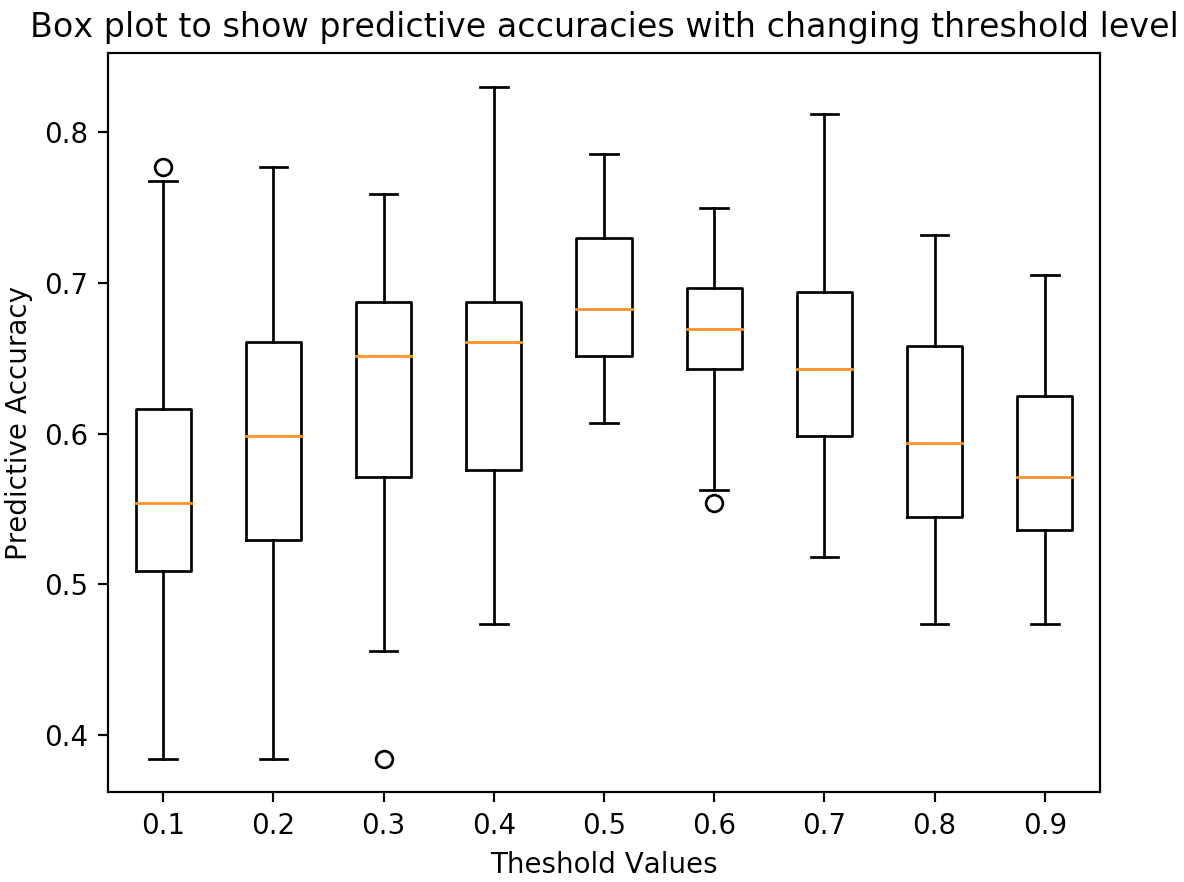
\includegraphics[scale = .40]{thresh}
\caption{Box and Whisker Plot to show different testing threshold values and their classification accuracies over 50 runs} 
\end{figure}

%%%%%%%%%%%%%%%%%%%%%%%%%%%%%%%%%%%%%%%%%%%%%%%%%%%%%%%%%%%%%%%%%%%%%%%%%%%%%%%%%%%%%%%%%%%%%%%%%%%%%%%%%%%%%%%%%%%%%%%%%%%%%%%%%%%%%%%%%%%%%%%%%%%%%%%%%%
The next test performed was using different selection methods. As the selection type is also a parameter, this increased the flexibility of the model. This is because I was able to create another selection mechanism, \textit{select\textunderscore best} to train and test the model. This selection function selected the best two individuals in the population every single time. The expectation of this was that when training the model, it would plateau off as the fitness values would start to converge to a fitness value similar to the parents, therefore converging at a local optimal solution. This did occur as can be seen in Figure 6  which compares the best current fitness in the population when using tournament selection and select best. 
\begin{figure}[h]
\centering
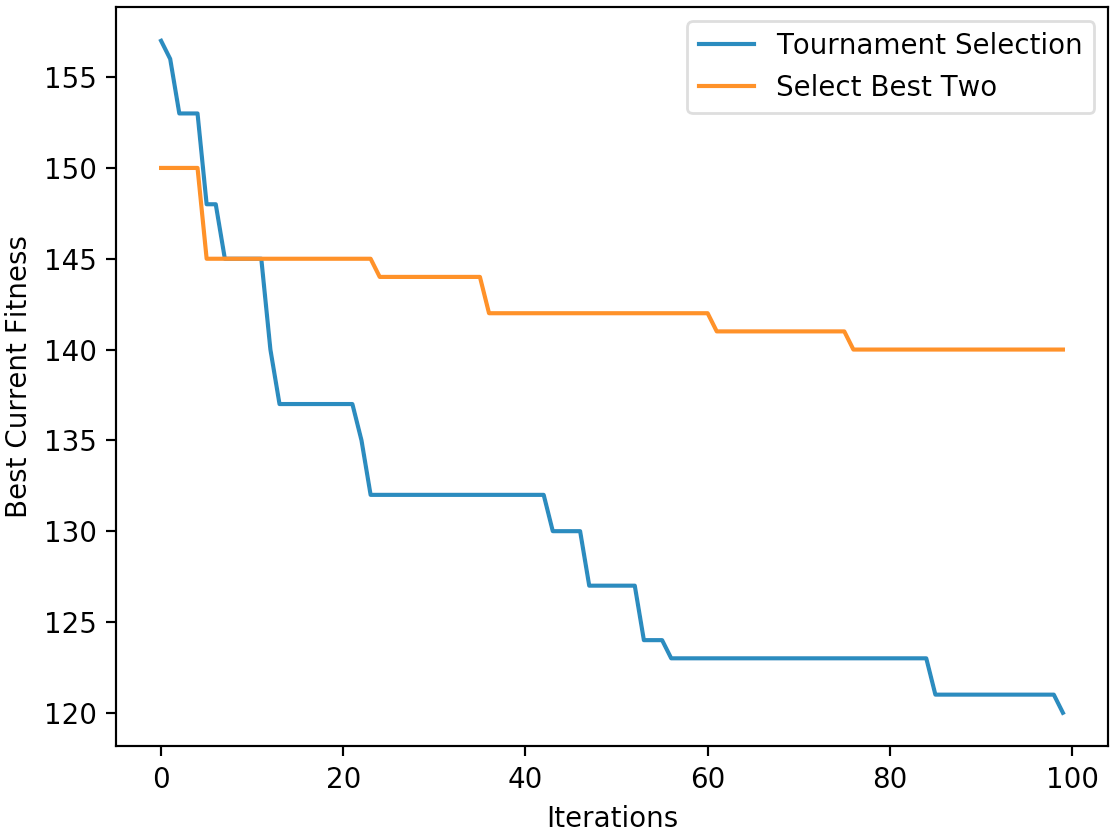
\includegraphics[scale = .40]{learning}
\caption{Line graph showing different parent selection methods and their learning fitness values. } 
\end{figure}
%%%%%%%%%%%%%%%%%%%%%%%%%%%%%%%%%%%%%%%%%%%%%%%%%%%%%%%%%%%%%%%%%%%%%%%%%%%%%%%%%%%%%%%%%%%%%%%%%%%%%%%%%%%%%%%%%%%%%%%%%%%%%%%%%%%%%%%%%%%%%%%%%%%%%%%%%%
Another parameter that could be tuned was the maximum number of iterations allowed before the model terminates. This involved using a variety of different maximum iteration values, to see if this made any difference to the predictive accuracies. In theory, if there were too few iterations, then the model would not be able to learn sufficiently. If there were too many iterations, then there is a possibility that learning would eventually stop, and that this would be very computationally expensive to try to find an optimal solution to the problem. Alternatively, learning would continue until an optimal function was found, however this posed the risk of the model overfitting the data. When using 10 and 100 as the parameter values, the GP appeared to still be learning (see Appendix E) . When the maximum iterations were 1000 or 2000, the model showed signs of convergence, and eventually stopped learning as quickly. While it may look like the model was no longer learning at all, until a termination criterion is met, the model would continue to search the search space for an optimal solution.

Through the use of software testing, using methods such as white and \textit{black box} testing, both the models made were successful and were able to predict whether a company would be likely to go bankrupt or not within one year. By using software testing, it enabled me to ensure that the models made were learning correctly. Through experimentation, I was able to determine more optimised parameters for both models which could be used to compare the models against each other. To make both models more user friendly, the configuration files were used to alter the parameters, which was a form of user acceptance testing. This means that, if a user wants to use both models, altering any source code would be unnecessary. Due to space limitations, I have only been able to mentioned some of the tests that were performed to tune the parameters of the model. \\
\subsection{ANN and GP Comparisons}\label{subsec:ANNGPC}
As part of the project, another aspect was to compare the developed two models to determine how well the GP performed against the ANN, in terms of time to find a solution, predictive accuracy and readability. \\

Firstly, I chose to compare the average time that it took the ANN and GP to train the model and test its predictive accuracy. To compare the two models, I used a line graph as this was a clear way to represent the comparisons.

\begin{figure}[h]
\centering
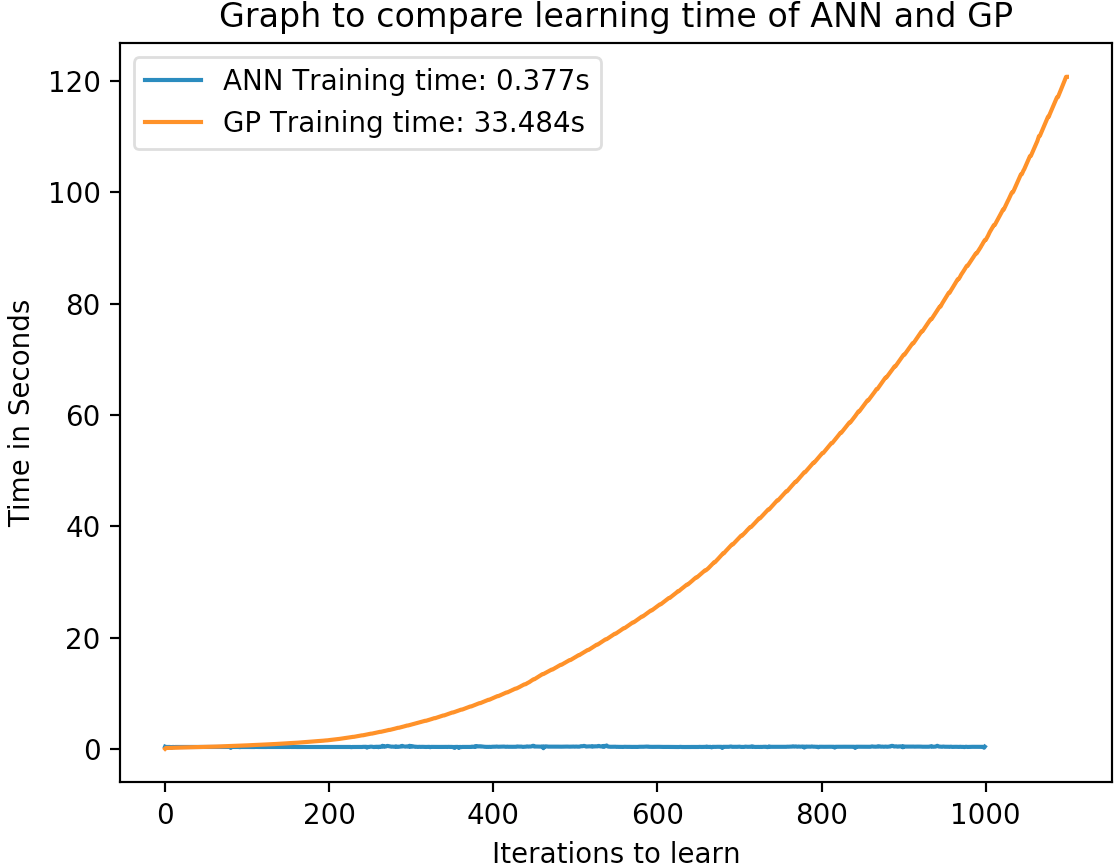
\includegraphics[scale = .45]{learning_rates}
\caption{Graph to show the learning rate over time seconds} 
\end{figure}
Since the ANN is a fixed sized model, it was expected that the time to perform 1000 iterations (epochs) to learn would remain relatively constant, as the size of the network never changes. 

The GP starts off at the same learning rate as the ANN. However after approximately 200 epochs, the time taken to learn starts to increase exponentially. By 1000 iterations, it takes approximately 120 seconds to run one iteration of the GP. When increasing the maximum iteration limit even further, the ANN times stayed relatively constant, while the GP time took even longer.  A possible reason for this is that smaller expressions with smaller trees can be evaluated much faster, as less computation is required to perform searching and evaluation. However as the trees undergo processes such as crossover, the new children trees can become much larger very quickly. In turn more recursion is required to search and evaluate the children produced which would increase the time to run one epoch. By 1000 iterations, the trees may have become exceedingly large, which means running one epoch will take significantly longer than when the population initially started. \\
%%%%%%%%%%%%%%%%%%%%%%%%%%%%%%%%%%%%%%%%%%%%%%%%%%%%%%%%%%%%%%%%%%%%%%%%%%%%%%%%%%%%%%%%%%%%%%%%%%%%%%%%%%%%%%%%%%%%%%%%%%%%%%%%%%%%%%%%%%%%%%%%%%%%%%%%%%
Another comparison that could be made was the readability between the two different models. One of the issues with ANNs is idea that it is known as a ``\textit{black box}" model. Although it is possible to look inside the model whilst it is learning, it is very difficult to understand exactly what is being changed within the network and how it is learning. Therefore studying the ANN structure can be very challenging. This is not the case with the GP. Whilst the GP is learning, because the individuals are mathematical expressions, tracking every single stage of the GP from start to finish is possible. This means that should someone want to look into the model whilst it is training, the expressions being selected, crossed over and mutated can be viewed. As a result, when the final solution is obtained, a readable function is produced and the user will know exactly how this solution has developed based on the starting population. \\

Finally, I also decided to compare the predictive accuracies of both models, based on their respective optimal parameters. Throughout the testing stage, I hypothesised that the ANN would outperform the GP in terms of predictive accuracy. To represent both results, an ROC curve was used. This  determined how likely the results produced were due to chance. 
\begin{figure}[h]
\centering
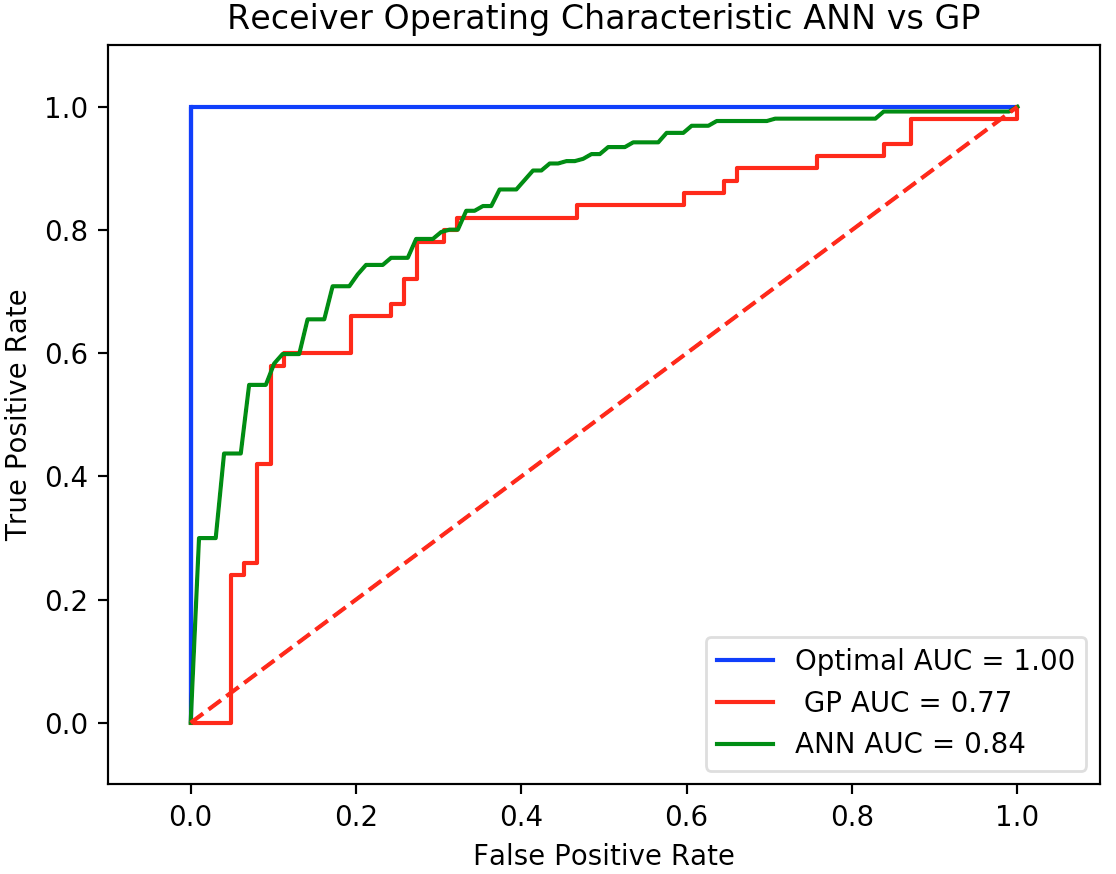
\includegraphics[scale = .50]{rocanngp}
\caption{ROC curve comparing the performance of ANN and GP. The Area Under Curve (AUC)  evaluates the performance of a classifier, where a probability of 1 is the optimal under the curve for a perfect classifier. Red dashed line signifies total randomness as a benchmark at 0.5.  } 
\end{figure}
%%%%%%%%%%%%%%%%%%%%%%%%%%%%%%%%%%%%%%%%%%%%%%%%%%%%%%%%%%%%%%%%%%%%%%%%%%%%%%%%%%%%%%%%%%%%%%%%%%%%%%%%%%%%%%%%%%%%%%%%%%%%%%%%%%%%%%%%%%%%%%%%%%%%%%%%%%
Looking at Figure 8, the ROC curve compares the ANN and GP true and false positive rates. The ROC shows that the area under the curve for the ANN and GP were 0.84 and 0.77 respectively, indicating that both classification models produced relatively strong models. In terms of their predictive accuracy, the ANN on average was closer to the optimal area under the curve indicating that on average, using the testing dataset, it was able to classify 84\% of the companies into the correct classifications, and 77\% for the GP. What can also be noted is that both of the models are a significant distance from the dashed red line, indicating the neither model achieved their results purely by chance. \\

Overall, after comparing some of the factors between the two optimised models, the ANN was generally superior to the GP, in terms of predictive accuracy and performance, although this does not mean to say that the GP performed poorly. Compared to the research conducted by Altman, who achieved 95\% predictive accuracy with his MDA model, the ANN and GP failed to meet this criterion. This could be due to the fact that he used a completely different dataset. Another factor could be because his data set did not include nonlinear data, which my dataset does. His research indicated that if the data was not linearly jointly distributed, then it was erroneous. Even though the models created perform worse than Altman's MDA model, they were able to handle nonlinear noisy data and still get between 70 - 85\% accuracy. 
Part of the reason the ANN may have performed so well was due to the fact that the ANN used a fully optimised library. This could mean that some of these optimised functions being used within the ANN library helped it to achieve better predictive results. 
Not only that, but to help improve the results further, the use of K-Fold cross validation was used which found the optimal parameters for this one part of the model. 

When developing  the GP, only the 4 basic mathematical operators were used. These may not necessarily be the wrong operators to have used, but more operators such as \textit{sin, cos} and \textit{log} could have also been used. Through using these, it is possible that an optimal solution produced, whilst more complex, would also give a higher predictive accuracy on the hold-out dataset.  Secondly, as a maximum depth limitation was not strictly enforced, after 1000 iterations, the GP started to become computationally expensive to keep running, even though learning had not finished. This meant that much larger solutions were constantly being checked, rather than smaller solutions which may have potentially had a better fitness. This effect of the trees getting very large very quickly is called \textit{bloat}. If there was a depth cap, then extremely large trees produced could have been removed to ensure that the performance was not affected. Finally, a possible reason that the GP did not perform as well as it could have is that since manual testing was performed to compute the best parameters, they may not have truly been the optimal parameters for the GP. This is something to consider as this was completed successfully for the ANN. \\

As these models are relatively dissimilar, the number of comparisons that could be made between the two models had to be relatively generalised to the two models as a whole, rather than being able to compare very specific parts of each model. By comparing the performance of the models, it was clear that the ANN stayed consistent in the time it took to learn due to its fixed size, unlike the GP which slowed down exponentially. The ANN also gave a better predictive output as the benchmark, using the official data set, augmented through parameter optimisation. However, the predictive accuracy was not significantly greater than the GP, and through the use of methods such as KFCV, the predictive accuracy could possibly surpass the ANN. 
\section{Future Work}\label{sec:FWC}
Throughout this project, I have learned many new concepts, ways of thinking, and how to use machine learning to approach the problem of binary classification to predict CB. There were parts of the project that were achieved very successfully and parts that may be improved upon for future work.  Due to time restrictions, there were several other features that each model could have used, which could have improved the development of each model.

Firstly, the ANN was built using a library, rather than from scratch, whereas the GP was built without the use of optimised libraries to help give better results. To make the models more comparable, the ANN could be created without the use of a library such as \textit{Sklearn}. Secondly an optimised library such as \textit{PyEvolve} or \textit{DEAP} could be used, to develop the genetic program. The reason that I have suggested this, is that more models could then be compared, against 2 ANNs and 2 GP, in order to compare their accuracies, efficiencies, and the possible causes for these changes in predictive accuracies. 

Furthermore, when developing the genetic program, if there was more time, a maximum tree depth would be enforced more strictly. Through crossover and mutation, the trees that are built can start to grow very quickly, especially when the crossover node has been selected higher up in the tree. As Figure (?) shows, this also means that the larger the tree, the more computationally expensive it is to evaluate. By imposing a maximum tree depth on any trees created, this would have several benefits. Firstly, it would reduce the computation time significantly as only children that fit within this maximum depth would be produced. In turn, the solutions produced would also be much smaller, but just as effective and could produce an optimal result. This also means that when training a model, the maximum iteration counter could be significantly larger, as this would not affect the computation time at all, as all the solutions would be much smaller.
Another factor that could be avoided in the future would be to not include a function that requires the building of a list of nodes to store the trees. To select a random node, rather that selecting from a list, this could be done directly via the tree itself. which would require less computation than building the tree, a list of nodes and selecting then selecting a node from the list of nodes. This in turn would help to improve the performance of the model.  

Next, when the optimal function produced is returned, the function produced could be pruned. Currently, the expression may be very large, which is not be straightforward to read. One way that this could be fixed in the future would be to prune the optimal expression, which evaluate any sub-expressions, and therefore cut down the total size of the function, whilst maintaining its original accuracy. This would make for a much better formulated function which would be easier for a user to use. 

Whilst testing the GP, only one type of crossover and mutation was implemented. Although this was sufficient, to allow more testing to occur, other crossover methods could be implemented. For example, \textit{size-fair crossover} could be used, which would help control the tree size by proportionally selecting a random subtree for parent one, but the same sized subtree for parent two. For mutations, a \textit{hoist mutation} or a \textit{shrink mutation} could be implemented. These could then be used with the crossover methods to help create more tests, which may be far better than just using the standard node replacement mutation that was used. 

Finally, for the datasets used, it was only American companies that were considered. In the future, data from other economies could be used, for example, from the British economy. This would provide score for more testing to be completed, to see if the current models could predict as accurately for companies from other countries. By having data from other economies, it could also potentially be used to make GP that could be applied universally, such that any company from around the world would be able to use the function to get a prediction and a classification. \\

Overall, if there was more time, many features could be inserted or adapted to make the development and usability of the genetic program potentially better, and more accurate.

\section{Reflection and Conclusions}\label{sec:Refl}
In the beginning stages of the project, I feel that the research completed was mostly done well, as I gained sufficient knowledge about this general topic, and some of the possible methods that had been used to approach this particular problem. A challenge I initially faced was finding enough research on genetic programming for binary classification. There were many research papers on the use of artificial neural networks and the use of genetic algorithms for binary classification and CB prediction, while there was not as much research for the use of expression trees to approach this task or to find an optimal function that could be applied to any given financial data. Overall I think that the research was relatively successful as it gave me a strong starting point about what to expect from this type of project, and what kinds of results I should be looking for. This also helped to make a realistic, achievable initial project specification which would include main features of each of the models to be developed.

Making the ANN design specification was a relatively straight forward process, as there were many research papers which discussed how they used ANNs to approach this problem. In turn, I was able to plan how each of the parts of the ANN would be constructed and why these choices were made. Since this type of model had been developed numerous times in the past, I decided to make this ANN a benchmark, where I could make an optimised model which could be compared against the other model that I was going to make, the GP. 

The process for designing the GP took longer, as there was a lot more to be achieved since GPs usually have a much longer process (see Figure 2). One of the big challenges I faced was data representation. The reason for this is that there were many different ways each section could have been represented. Since the aim was to produce an optimal function, I thought that the best way to represent this for a user, would be through infix notation - notation that most people are familiar with. On the other hand, research showed that each stage in the GP could have been represented using only a binary tree structure, though I felt this was unnecessary as it would have involved a lot of needless computation. 

Overall the creation of the design specification was very successful. I felt that the specification was plentiful and realistic enough such that the project could be completed with the requirements met, whilst still challenging me throughout the development and testing phases. \\
%%%%%%%%%%%%%%%%%%%%%%%%%%%%%%%%%%%%%%%%%%%%%%%%%%%%%%%%%%%%%%%%%%%%%%%%%%%%%%%%%%%%%%%%%%%%%%%%%%%%%%%%%%%%%%%%%%%%%%%%%%%%%%%%%%%%%%%%%%%%%%%%%%%%%%%%%%

By using the \textit{Sklearn} library, the development and implementation of the ANN was relatively uncomplicated. The reason for this is because to execute the ANN model, there were only a few crucial components required to construct it, fit the data to the model, and use the trained model to test the predictive accuracy. In turn, this allowed me to exploit the library functionality to enable tests to be performed on this model. This included running the model once on a small static data set to determine if the model was in fact learning, before using the full data set to run the classification model. Once this was achieved, using the \textit{cross\textunderscore val\textunderscore score} functionality, I was then able to split the data into training and testing datasets using 10-Fold cross validation and find the optimal number of nodes that would produce the best predictive accuracies. Through the testing completed, I could successfully return the optimal number of layers, and the optimal number of nodes required for all the layers. Through the 10-Fold cross validation, the optimal average predictive accuracy was also determined.

Due to the variety of parameters that could be applied to the \textit{MLPClassifer}, I was able to exceed the expectations of the ANN by being able to apply different activation functions and different learning functions that could be combined together to find the most appropriate methods used to make the ANN successful. This was not part of the project or the design specification, however, as these facilities were available, I was able to experiment with these. Using these enabled more experimentation to be performed than initially planned as these functions were already pre-built functions. 

As I built the GP without the aid of any libraries, the majority of the programming aspect was completed here. Overall, by using the design specification as a template model, I was able to successfully develop the GP which produced an optimal expression to predict CB. Throughout this stage, I did encounter problems which eventually were handled. For example, although converting infix notation to prefix notation by hand was straightforward, applying this into a function was very challenging, and I found myself wasting too much time trying to make it work. Eventually I was able to find tutorials on how to convert infix to prefix notation, which I was then able to follow, and adapt to fit the needs of the GP model. By the end of the development phase, all of the issues that needed to be fixed, were completed, and the model was able to learn on the training set and produce an optimal function. As the two example functions produced show, the X1 KPI - \textit{working capital / Total Assets} had been filtered out of \textit{optFunc1}, which proved that this variable had no effect on the predictive accuracy of the model, and was not needed when random constants were used. However all the KPIs were required when random constant variables were not included. This met the project specification by showing which KPIs were crucial in all environments and which ones were not.\\

Looking back at the testing aspect of the models developed, I feel that individually each model was tested well, to establish any errors during the development which were not caught, which is why unit testing proved to be very useful. These flaws allowed me to go back through the code to fix any outstanding errors that may have occurred. Due to time restrictions, I was able to handle certain errors and fix them entirely, however for others, this was not always  possible. For example, if the GP initial maximum depth exceeds a certain limit, the model indicates that the depth has exceeded the maximum depth limit, and exits the model, indicating that the user should make the initial depth smaller. Another error that could have been avoided was the conversion of prefix to infix notation. Usually this worked, however very occasionally, the child would be formed incorrectly. In turn this caused the model to crash. Therefore to handle this error, the broken child was removed and replaced with a new expression, to allow the program to keep running. Finally to meet more of the specification, I created a configuration file for the user to be able to put in their inputs, so that a user can use their own configurations to let the model learn without having to manually change any of the source code. 
\\\\
To conclude, this project has been successful in all aspects. I was able to use the research I found to create a project specification. This included making two detailed plans for the models that were to be made. Using these design specifications, I was then able to make the models using the Python programming language, using \textit{Sklearn} as to design the ANN to be an optimised model to compare the GP against. Using the models that were made, I was then able to test the models to ensure they worked through methods such as unit testing, performance testing, and classification accuracy, and came to the conclusion that both models were fit for this particular problem. If there was more time, certain aspects of the project would have been changed, to make this project more successful, however with the time that I was given, I feel that the models that were made produced results that were comparable to techniques that are currently being used in industry to predict the likelihood of corporate bankruptcy. \\
***Note to reader. To execute the ANN and GP model, please refer to Appendix B and C respectively. 
\cleardoublepage
\bibliographystyle{agsm}
\bibliography{/Users/carlsaptarshi/Desktop/gp/gp/references/refs.bib}
\cleardoublepage

\appendix
\section{Use of Key Performance Indicators}
Using Altman's research, he demonstrated the use of 5 KPIs which were used as the inputs for both the models that were developed. This meant that each of these ratios played a significant role in determining the performance of a company. \\
\\
\textbf{X1} - Working Capital / Total Assets \\
\textbf{X2} - Retained Earnings / Total Assets\\
\textbf{X3} - Earnings Before Interest and Tax / total Assets\\
\textbf{X4} - Market Value of Equity / Total Debt\\
\textbf{X5} - Sales / Total Assets\\
\\
\textbf{X1} - This is a measure of the net liquid assets of the firm relative to the total capitalisation. A firm experiencing consistent losses whilst operating will have shrinking current assets in relation to total assets \cite{ref-six}. \\
\\
\textbf{X2} - The essential idea here is based on the age of the firm. Younger firms ave had less time to grow and develop, and therefore had less time to accumulate profits. In turn, they are more likely to go bankrupt statistically speaking. \cite{ref-six}.\\
\\
\textbf{X3} - This looks at the productivity of the firm. The reason this ratio was selected was based on the ideas that if a company is more productive, they will tend to have more assets, and therefore would be less likely to fail, and vice versa. Therefore this ratio was very applicable in the area of CB \cite{ref-six}.\\
\\
\textbf{X4} - This is measure that is able to indicate the leeway that a company will have before it is said to be financially distressed, and could then lead to company insolvency.\cite{ref-six}.\\
\\
\textbf{X5} - This takes on a measurement about how management teams are able to cope in competitive environments. The more sales they make, the more assets they will also have. This works both ways, and can potentially lead to the collapse of a company if the company stops making sales.  \cite{ref-six}.

Overall, as these ratios show, they all play a crucial role in being able to predict CB within one year. They each give a vital role in determining the financial health of a company at any point in time. 

\newpage
\section{Executing the ANN using a Configuration File}

\textbf{CONFIG FILE ANN}\\
How to use:\\
Please enter the configuration details of how you would like to construct the artificial neural network the structure is as follows:\\
\\
   :param \textit{structure}: for every hidden layer, insert value for number of nodes per hidden layer, separated by a space\\
   :param \textit{learning\textunderscore method}: Learning Methods include - choice {[`lbfgs', `sgd', `adam']}\\
   :param \textit{test\textunderscore size}: percentage of dataset to test the network (value between 0 and 1)\\
   :param \textit{train\textunderscore size}: percentage of dataset to train the network (value between 0 and 1)\\
   -  please ensure that values do not exceed 1 or smaller than 0\\
   -  for more realistic predictions, use a training dataset percentage of size x and testing dataset size 1-x
   :param \textit{activation}: activation function to be used - choice {[`identity', `logistic', `tanh', `relu']}\\
   :param \textit{max\textunderscore iterations}: maximum number of iterations to be used before learning MUST stop.\\
\\
Example:\\
\textit{[DEFAULT] }\\
structure =  5 5 \\
learning\textunderscore method = lbfgs \\
test\textunderscore size = 0.2 \\
train\textunderscore size = 0.8 \\
activation = logistic \\
max\textunderscore iterations = 1000 \\
\\
save as config.ini within this directory and then execute model.
\\
\\
To execute the ANN, please use the ANN directory.\\
This contains \textit{cross\textunderscore validation\textunderscore ANN.py} to run KFCV on the ANN. This file can be built and run immediately. 
\textit{crossValRoc\textunderscore ANN} is used to make the ROC curves based on the optimal nodes found in \\
\textit{cross\textunderscore validation\textunderscore ANN.py}. \\
\textit{Train\textunderscore test\textunderscore split\textunderscore ANN.py} is used with configuration file to run TTS on the data set based on the users parameters. 

\newpage
\section{Examples of the GP in Verbose Mode}
This appendix is to show the reader how an example of a complete run of the GP looked like visually after the parents had been selected.  Please read each image from left to right. \\


\begin{figure}[h]
\centering
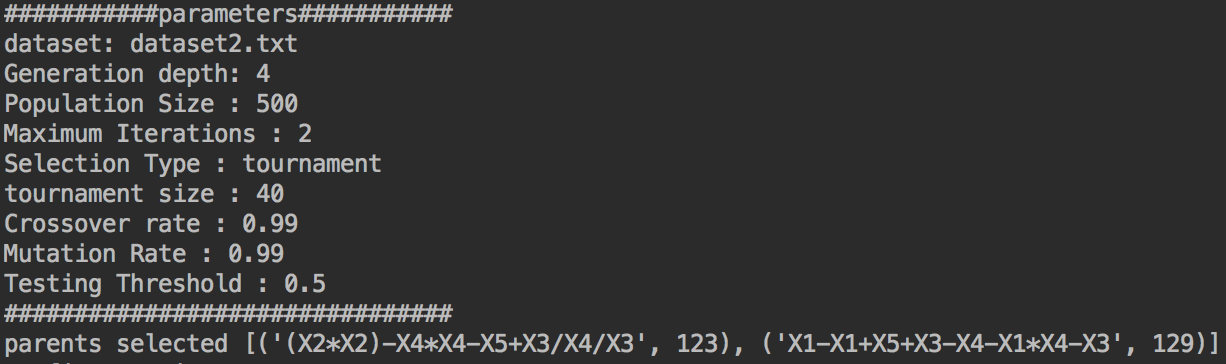
\includegraphics[scale = .60]{1}
\end{figure}
parent prefix:  [([`-', `*', `X2', `X2', `-', `*', `X4', `X4', `+', `X5', `/', `X3', `/', `X4', `X3'], 123), \\
([`-', `X1', `+', `X1', `+', `X5', `-', `X3', `-', `X4', `-', `*', `X1', `X4', `X3'], 129)]
\begin{figure}[h]
\centering
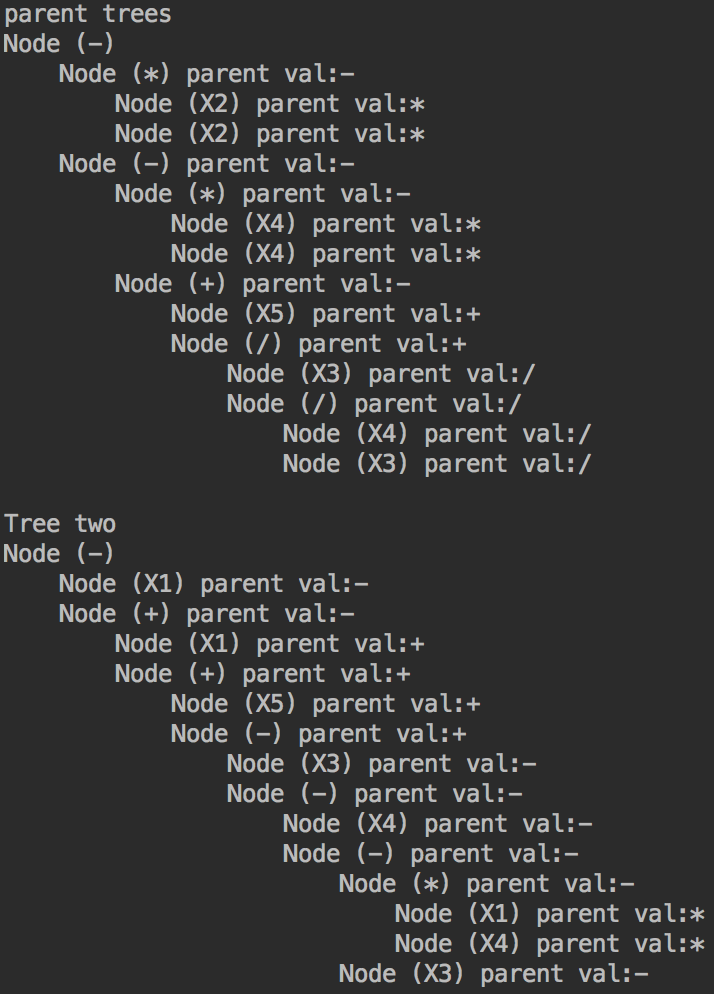
\includegraphics[scale = .60]{2}
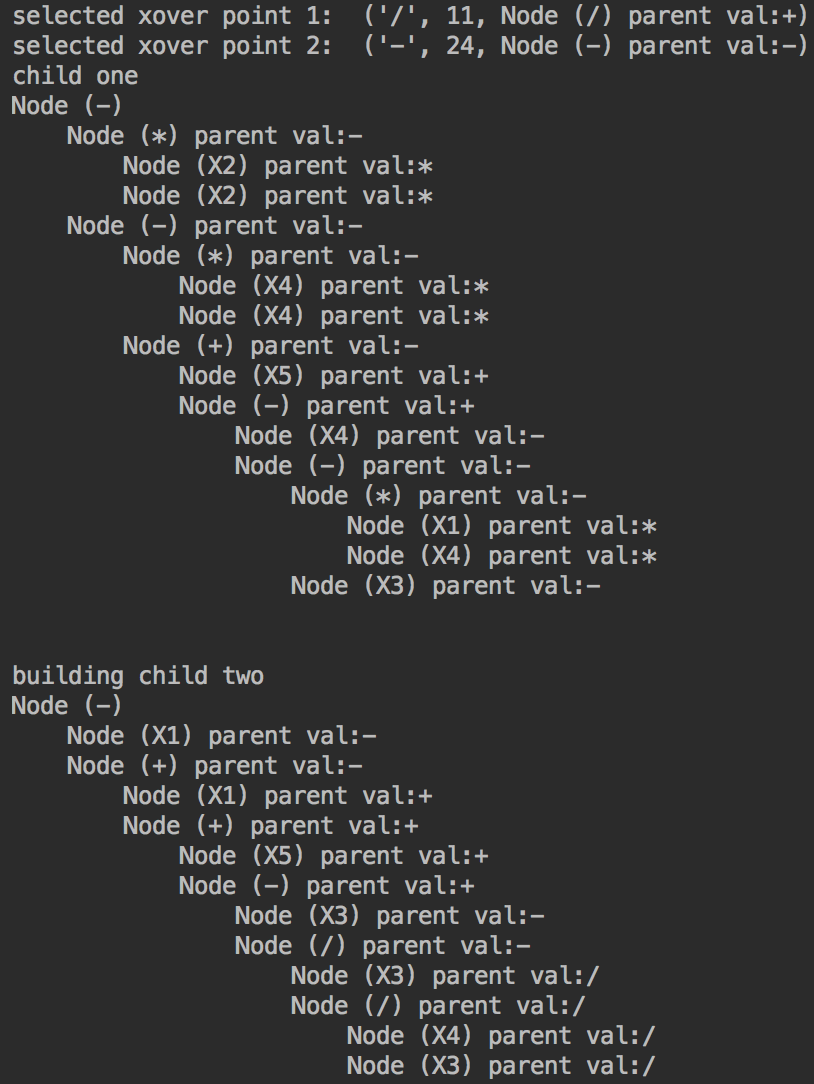
\includegraphics[scale = .60]{3}
\end{figure}

\newpage
\section{ROC curve to test GP and ANN}
\begin{figure}[h]
\centering
Genetic Program using TTS with 80\% training data and 20\% testing data:
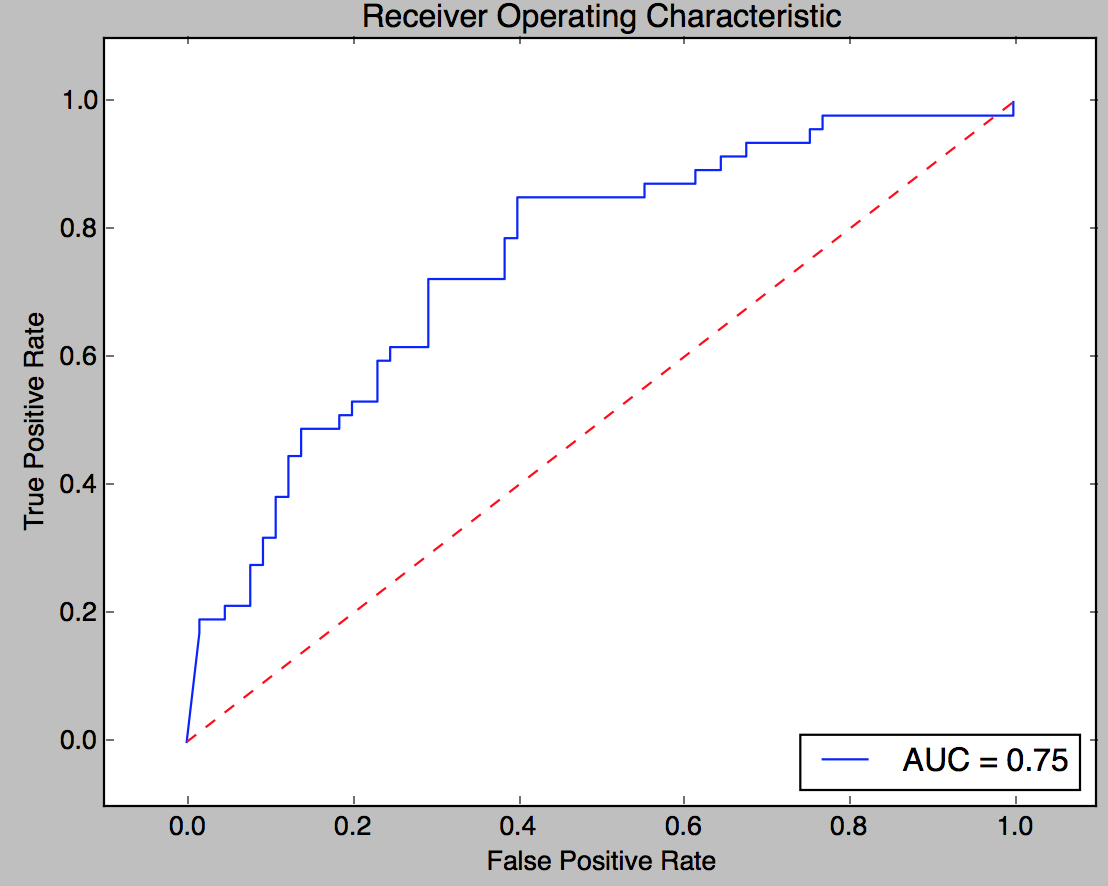
\includegraphics[scale = .40]{gp1}
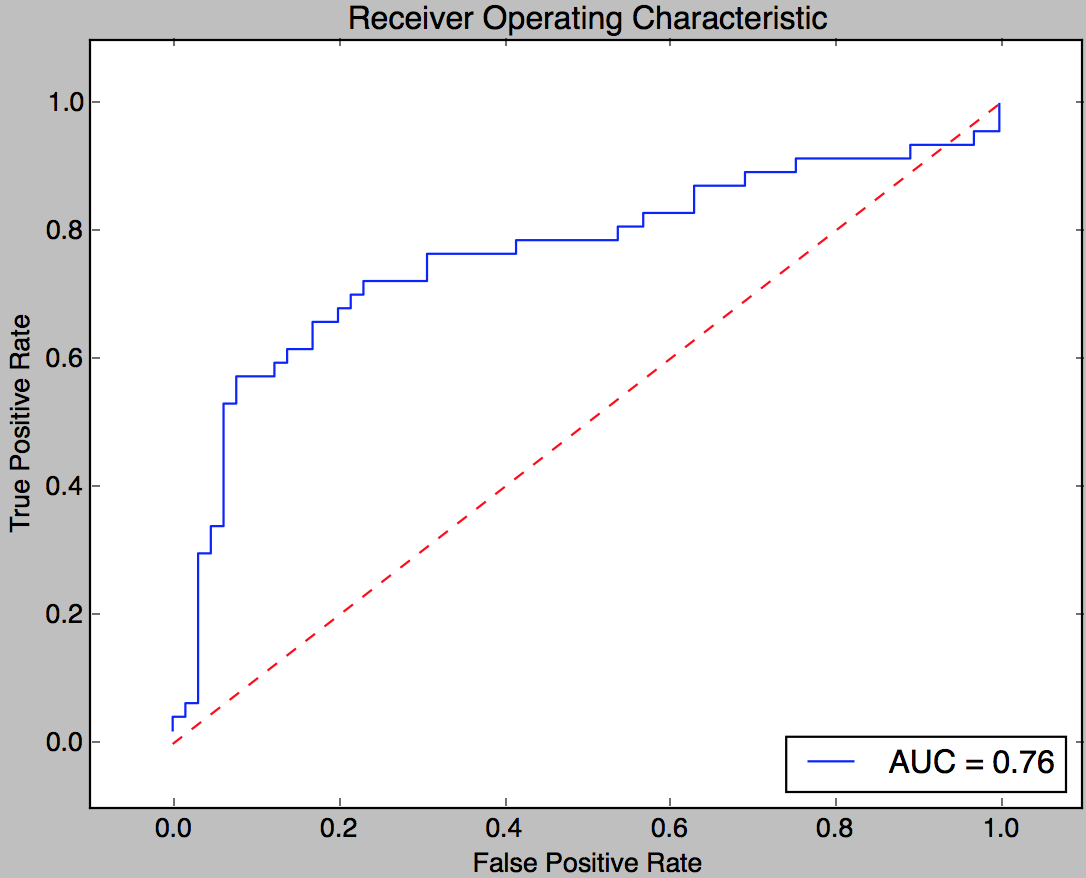
\includegraphics[scale = .40]{gp2}
\end{figure}
\begin{figure}[h]
\centering
ANN using TTS with 80\% training data and 20\% testing data:
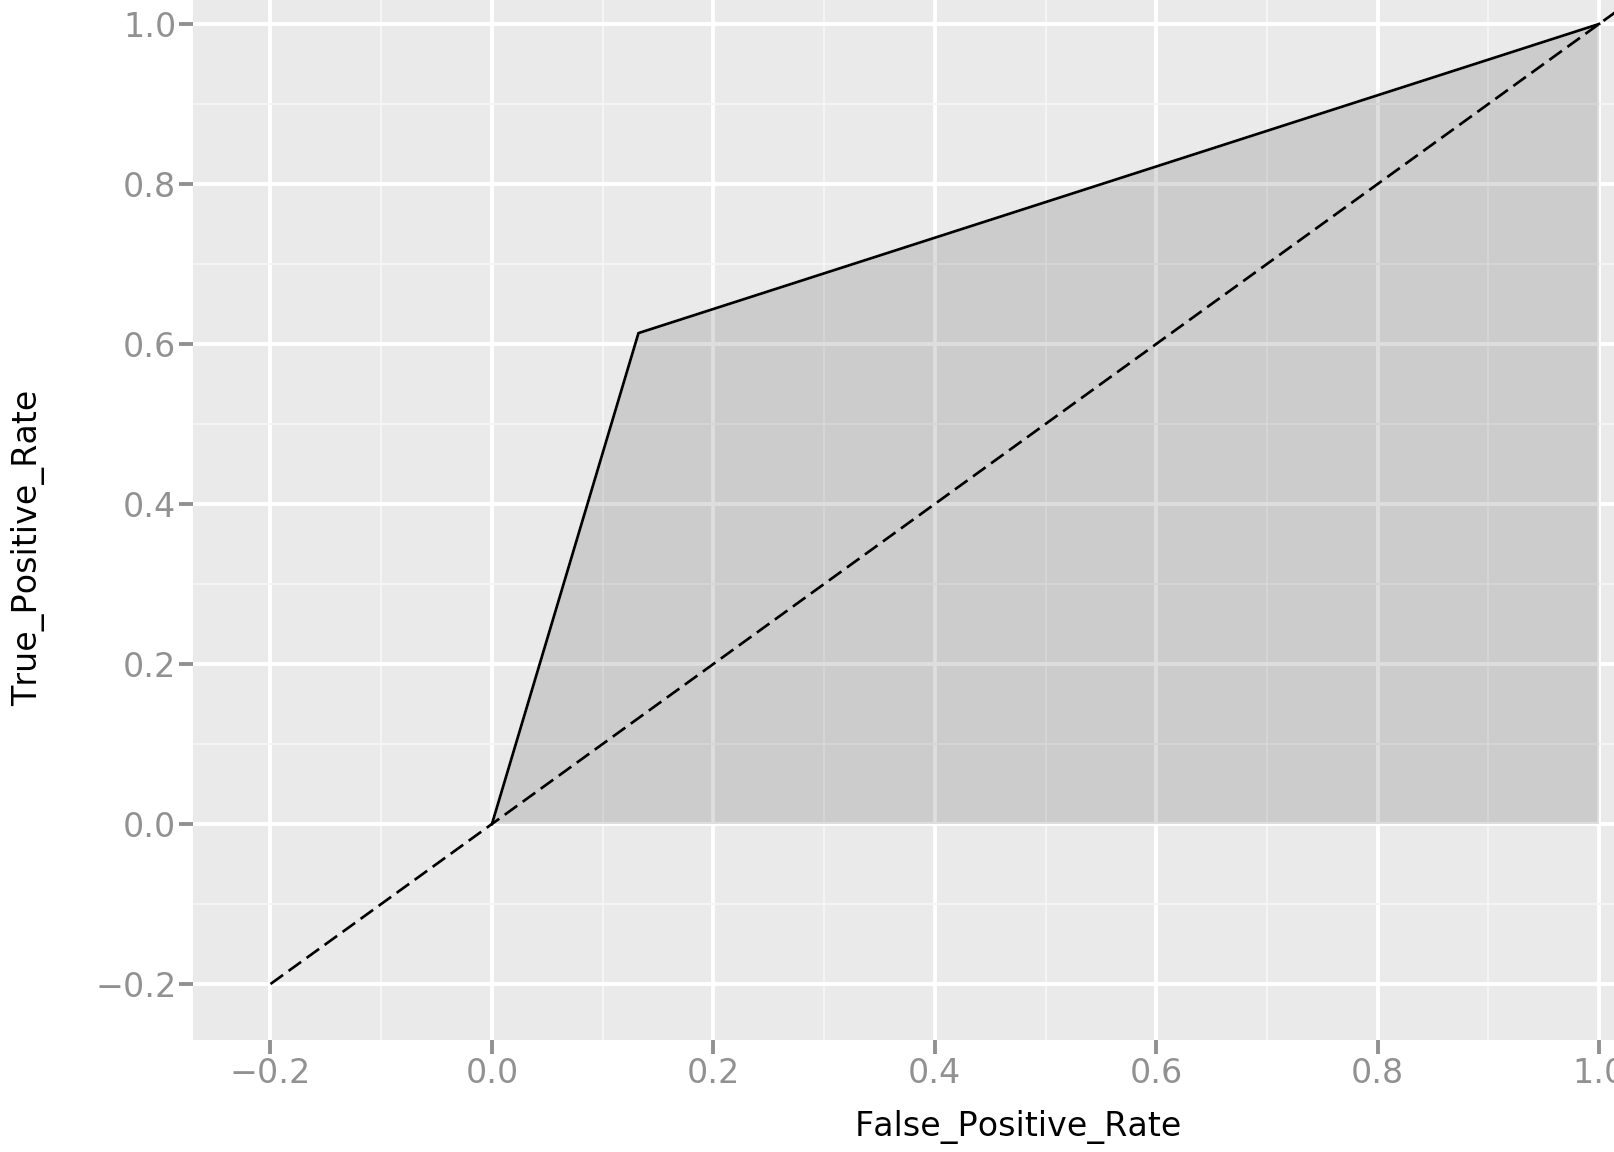
\includegraphics[scale = .30]{ann1}
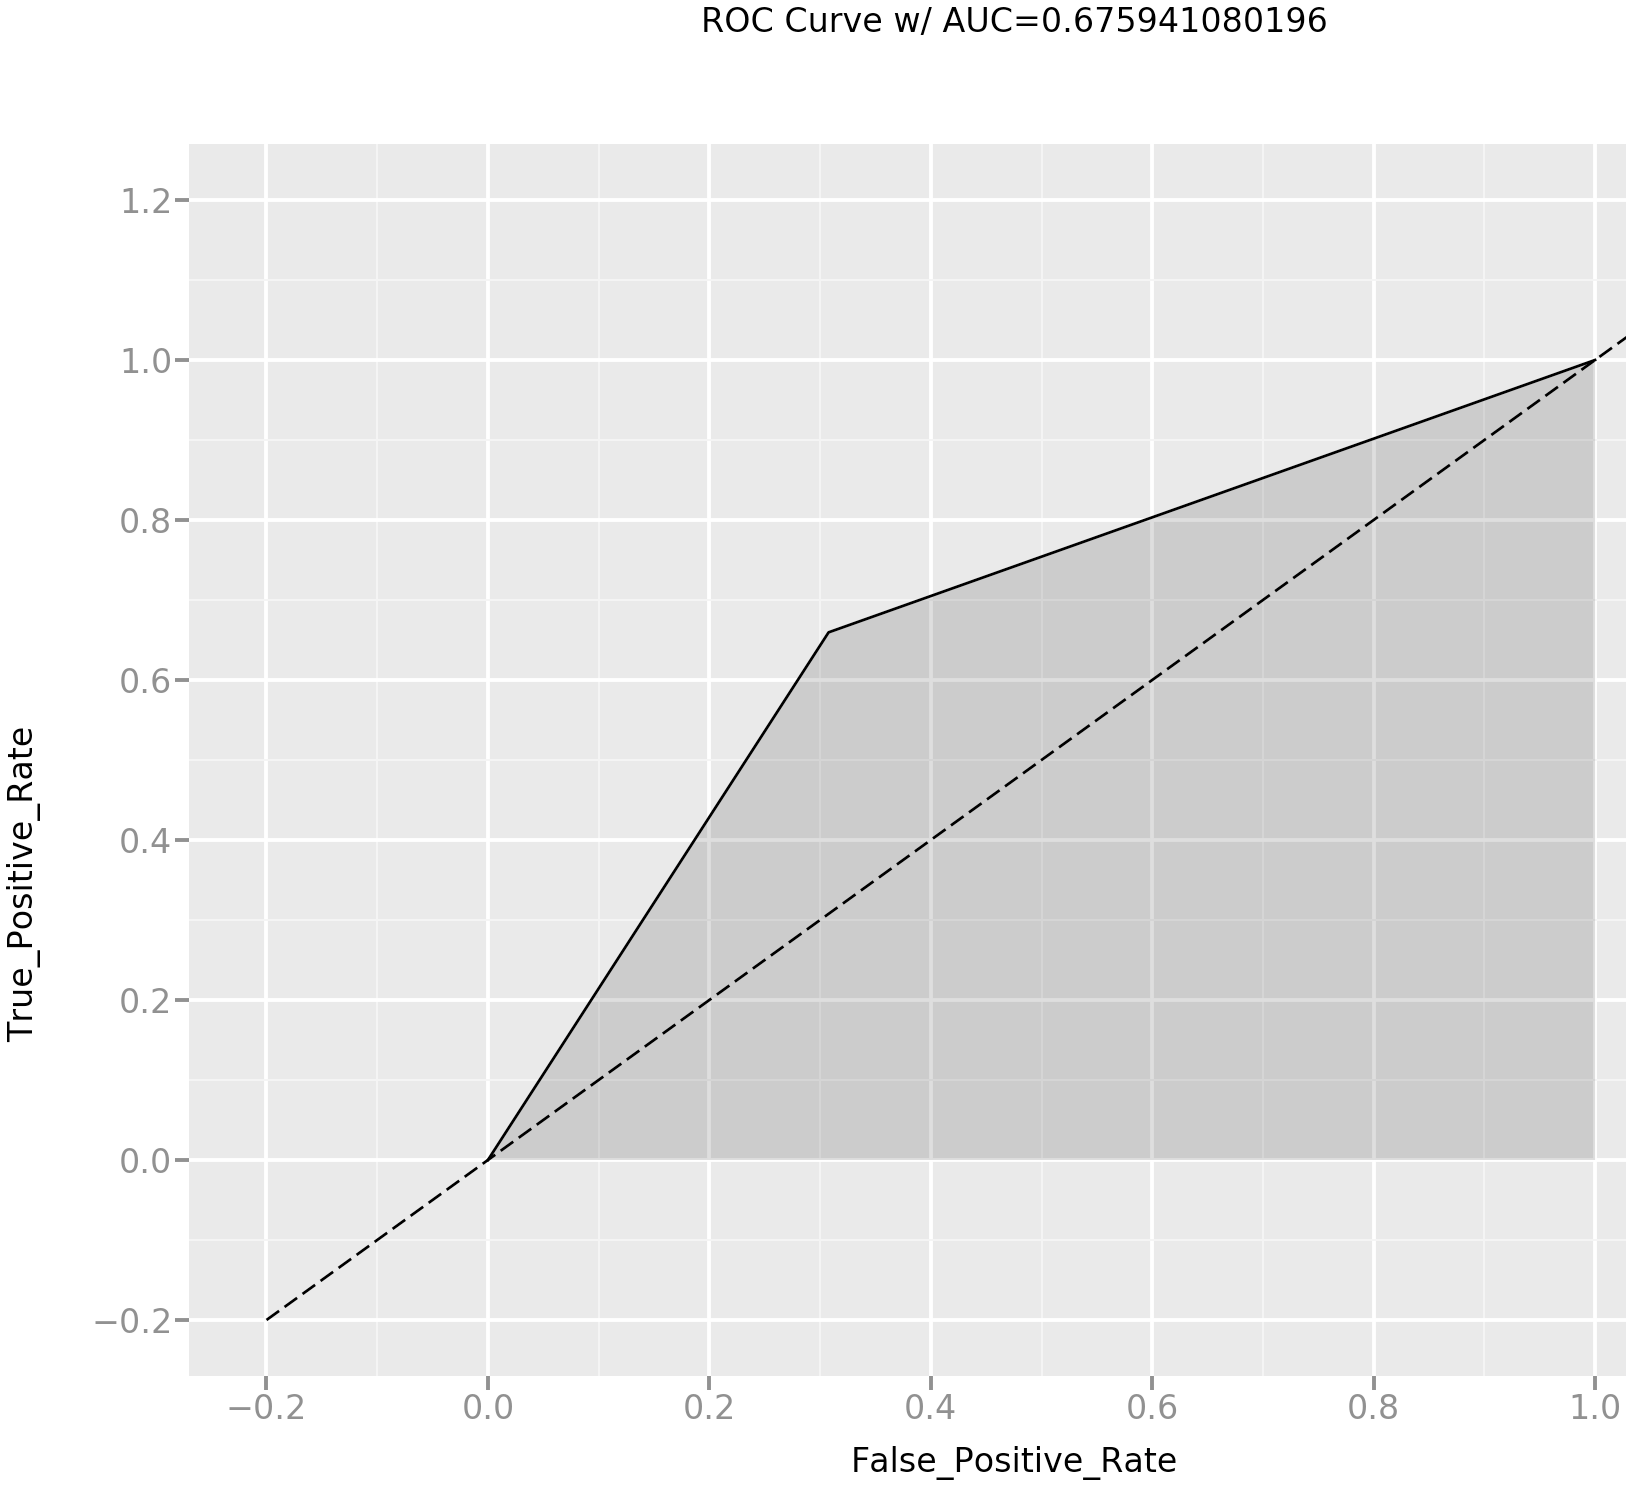
\includegraphics[scale = .25]{ann2}
\end{figure}


\newpage
\section{ROC curve to test GP and ANN}
\begin{figure}[h]
\centering
Genetic Program with 50 and 100 iterations of running the model:
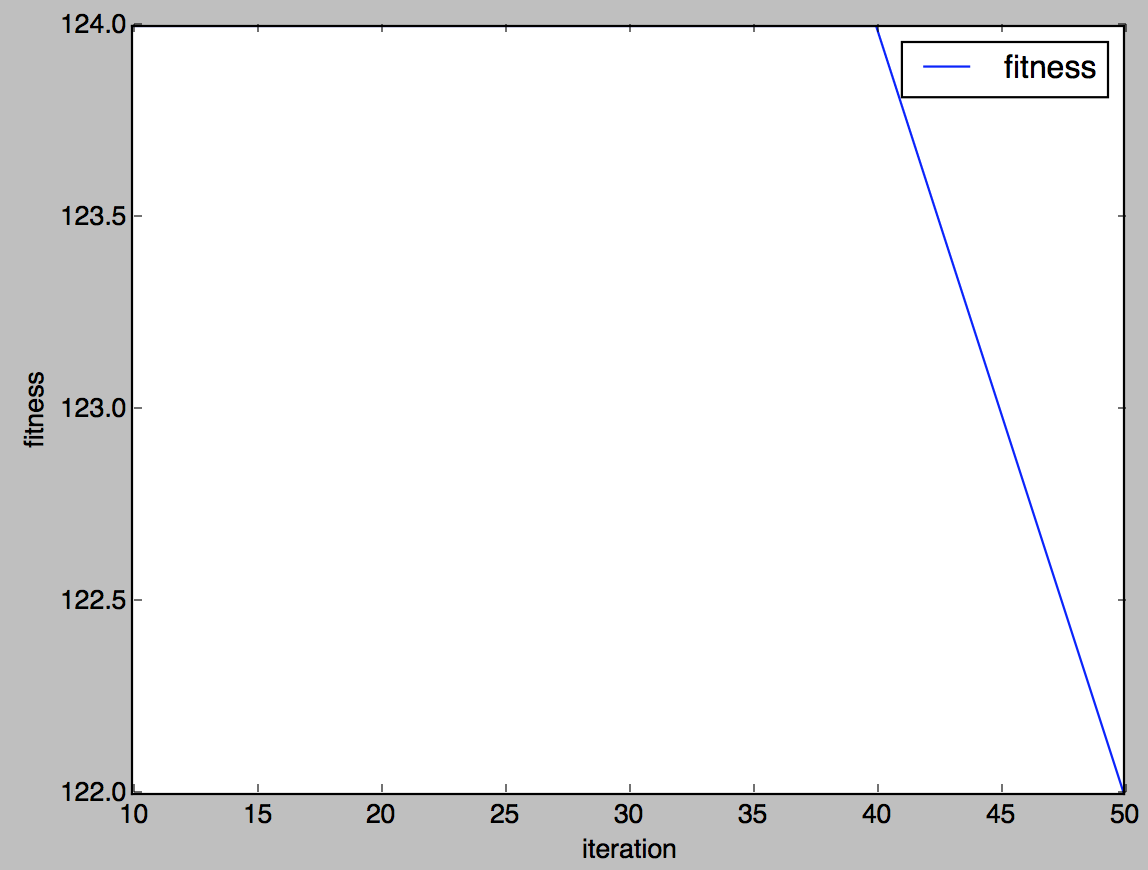
\includegraphics[scale = .35]{learn1}
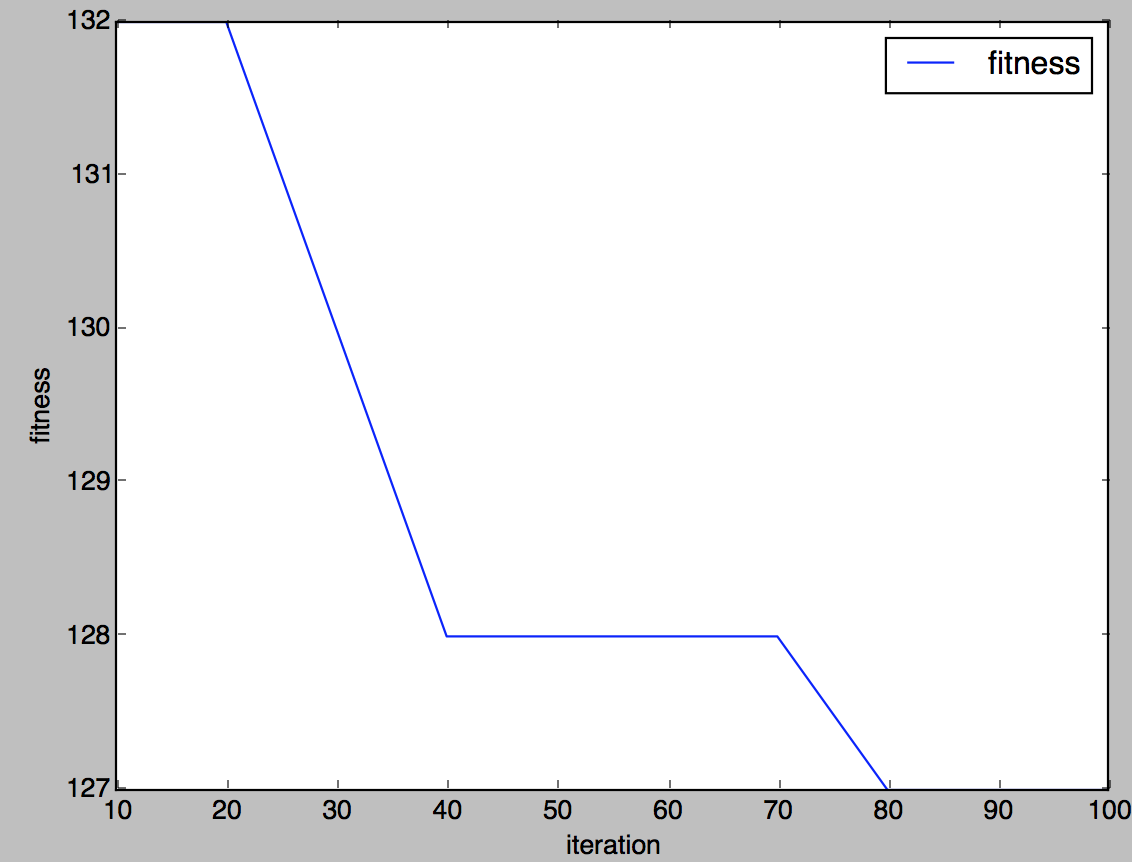
\includegraphics[scale = .35]{learn2}
After 50 iterations it can be seen that learning has only just commenced and the model is beginning to learn quickly. As can be seen, more than 50 iterations are needed for the model to learn sufficiently. After running the model for 100 iterations, the model is still learning as well, as no optimal solution has been found yet. That being said, learning began in the very early stages of this model. After 100 epochs, changes are still expected and the performance of this will not be effected as was seen in Section 5.2 Figure 7, the computation time only starts to increase after approximately 200 epochs.
\end{figure}
\begin{figure}
\centering
Genetic Program with 1000 and 2000 iterations of running the model:
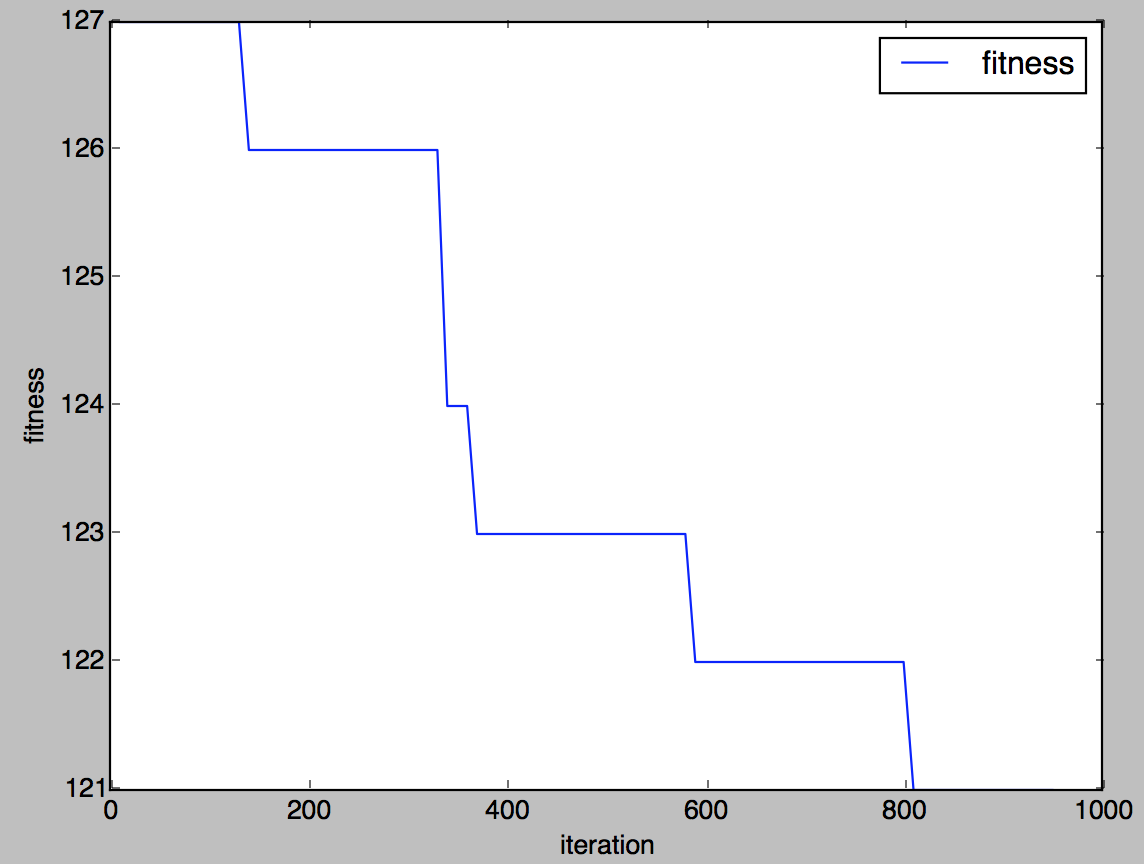
\includegraphics[scale = .4]{2k}
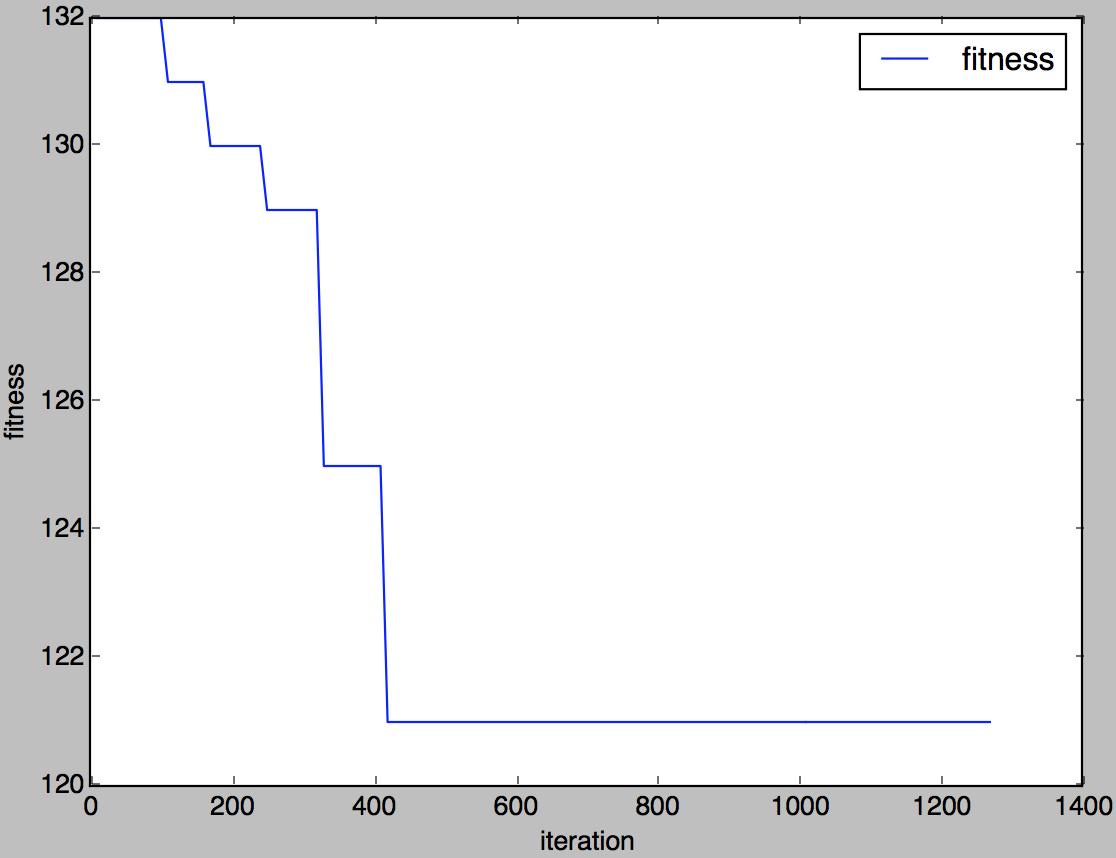
\includegraphics[scale = .4]{3k}
Approaching 1000 runs, the model is still learning as the fitness has reduced from 127 to 121. However in 1000 runs, the accuracy of the model has only increased by 1\%, whereas the computation time to achieve this extra 1\% has been significantly more. As expected when running 2000 times, the computation time started to increase too much, and the rate of learning had plateaued at approximately 450 epochs of this model. 
\end{figure}






\end{document}




